%%%%%%%%%%%%%%%%%%%%%%%%%%%%%%%%%%%%%%%%%
% The contents of this document are the copyright of Joseph Hale
%
% This Source Code Form is subject to the terms of the Mozilla Public
% License, v. 2.0. If a copy of the MPL was not distributed with this
% file, You can obtain one at https://mozilla.org/MPL/2.0/.
%%%%%%%%%%%%%%%%%%%%%%%%%%%%%%%%%%%%%%%%%

\chapter{Evaluation}
\label{Chapter7}

This chapter seeks to measure the effectiveness of the design proposed
in Chapters \ref{Chapter4}, \ref{Chapter5}, and \ref{Chapter6}. To do
so, this chapter will use four key benchmarks derived directly from the
research questions outlined in Section \ref{sec:research-questions}.

The benchmarks are as follows:

\begin{itemize}

    \item \emph{Move Tracking Accuracy}: How accurately can the design
    track the moves performed on the modified speedcube? (Section
    \ref{sec:move-tracking-accuracy})

    \item \emph{Compatibility with Standard Speedcubes}: How
    effectively can the design be deployed in a standard, non-smart
    speedcube without any permanent modifications or reducing the
    cube's performance? (Section
    \ref{sec:compatibility-with-standard-speedcubes})
    
    \item \emph{Move Tracking Granularity}: What other metrics can each 
    design provide (Section \ref{sec:move-tracking-granularity})?
    
    \item \emph{Competition Legality}: To what extent is the design
    compliant with existing competition regulations? (Section
    \ref{sec:competition-legality})
    
\end{itemize}


\section{Move Tracking Accuracy}
\label{sec:move-tracking-accuracy}

For the design to be usable it must be able to track the moves of a
traditional, non-smart speedcube. Furthermore, since untracked moves
render the final move sequence invalid unless manually reviewed and
corrected, it is critical that the design detect moves with high or
perfect accuracy.

While Chapter \ref{Chapter5} demonstrated a perfect detection of a
transmitted move sequence, this section seeks to explore the limits of
the software receiver. To do this, the receiver was subjected to a
battery of tests consisting of running several noisy synthetic audio
sequences (see Section \ref{sec:adding-realistic-noise}) through the
receiver algorithm with a variety of parameters and comparing the
detected move sequence to the one used to generate the audio.

The noisy synthetic audio samples used in this testing were engineered
to represent both the full range of face turns that could be performed
on the cube and the turn speeds of speedcubers that average 12-30
seconds per solve. To that end, the "demo alg" from Figure
\ref{fig:example-alg-audio} which sweeps through every possible
centerpiece state was rendered at 2 TPS and 5 TPS\footnote{Given a that
a typical speedsolver averages 60 moves per solve \cite{pochmann-hume}, 2TPS
corresponds to an average solve time of 30 seconds and 5TPS corresponds
to an average solve time of 12 seconds.} using the code shown in Figure
\ref{fig:code-generate-alg-audio}. Then, those two audio samples were
each augmented with the background noise of a quiet, normal volume, and
noisy speedcube (respectively the Gans 356, Gans X, and QiYi QiMeng
described in Section \ref{subsec:signal-to-noise-ratio}) using the
techniques discussed in Section \ref{sec:adding-realistic-noise} for a
total of 6 audio samples that serve as a basic cross-section of the
most common variations in cubes and turn speeds.

With this representative sample set of audio signals in hand, the
limits of the receiver could be tested. Each test comprised of setting
the three parameters of the receiver to a specific combination of
values (each chosen from a range of values determined emprically),
running all six audio samples through the receiver, then comparing the
detected move sequence with the actual move sequence for a percent
similarity calculation. The standard deviation threshold parameter
\code{stdv\_pct} (Section \ref{subsec:fine-tuning-threshold}) varied
through from 0.25 to 3 in increments of 0.25 for a total of 12 values.
The minimum threshold parameter \code{min\_thresh} (Section
\ref{subsec:fine-tuning-threshold}) varied from 50 to 550 in increments
of 50 for a total of 6 values. The window size parameter
\code{window\_size} (Section
\ref{subsec:ignoring-noise-when-extracting-move-sequences}) varied from
1 to 10 time steps in increments of 1 for a total of 10 values. In
total, the 12 standard deviation thresholds, 6 minimum thresholds, 10
window sizes, 2 turn speeds, and 3 cubes yielded 4,320 unique
combinations with which to test the receiver algorithm.

The insights gained from analyzing the resulting data are discussed in
the following subsections. Section
\ref{subsec:influence-cube-noisiness} explores the influence of cube
noisiness on detection accuracy. Section
\ref{subsec:influence-stdv-threshold} does the same for the standard
deviation threshold. Section \ref{subsec:influence-alt-min} covers the
minimum threshold. And Section \ref{subsec:influence-window-size}
reviews the window size. The turn speed factor is discussed in all
subsections as an additional angle for understanding each factor's
unique influence on detection accuracy.

\subsection{Influence of Cube Noisiness}
\label{subsec:influence-cube-noisiness}

The three cubes used for this analysis - the Gans 356, Gans XS, and
QiYi Qimeng - respectively represent quiet, normal, and loud speedcubes
(see Section \ref{subsec:signal-to-noise-ratio}). The louder speedcubes
were expected to cause more difficulties for decoding the transmitted
move sequence since they create more noise that may conflict with the
audible signal. Since all cubes produced more noise when turned at a
higher speed and there is less time for detection to complete, the
simulated turn speeds were also expected to experience inferior
performance during move sequence detection.

\begin{figure}
\caption{Perfect Detections by Cube}
\label{fig:perfect-detections-by-cube}
\begin{subfigure}{\textwidth}
    \centering
    \caption{Total number of perfect detections \\ (Aggregate of Figures \ref{fig:perfect-detections-by-cube-2tps} and \ref{fig:perfect-detections-by-cube-5tps})}
    \label{fig:perfect-detections-by-cube-total}
    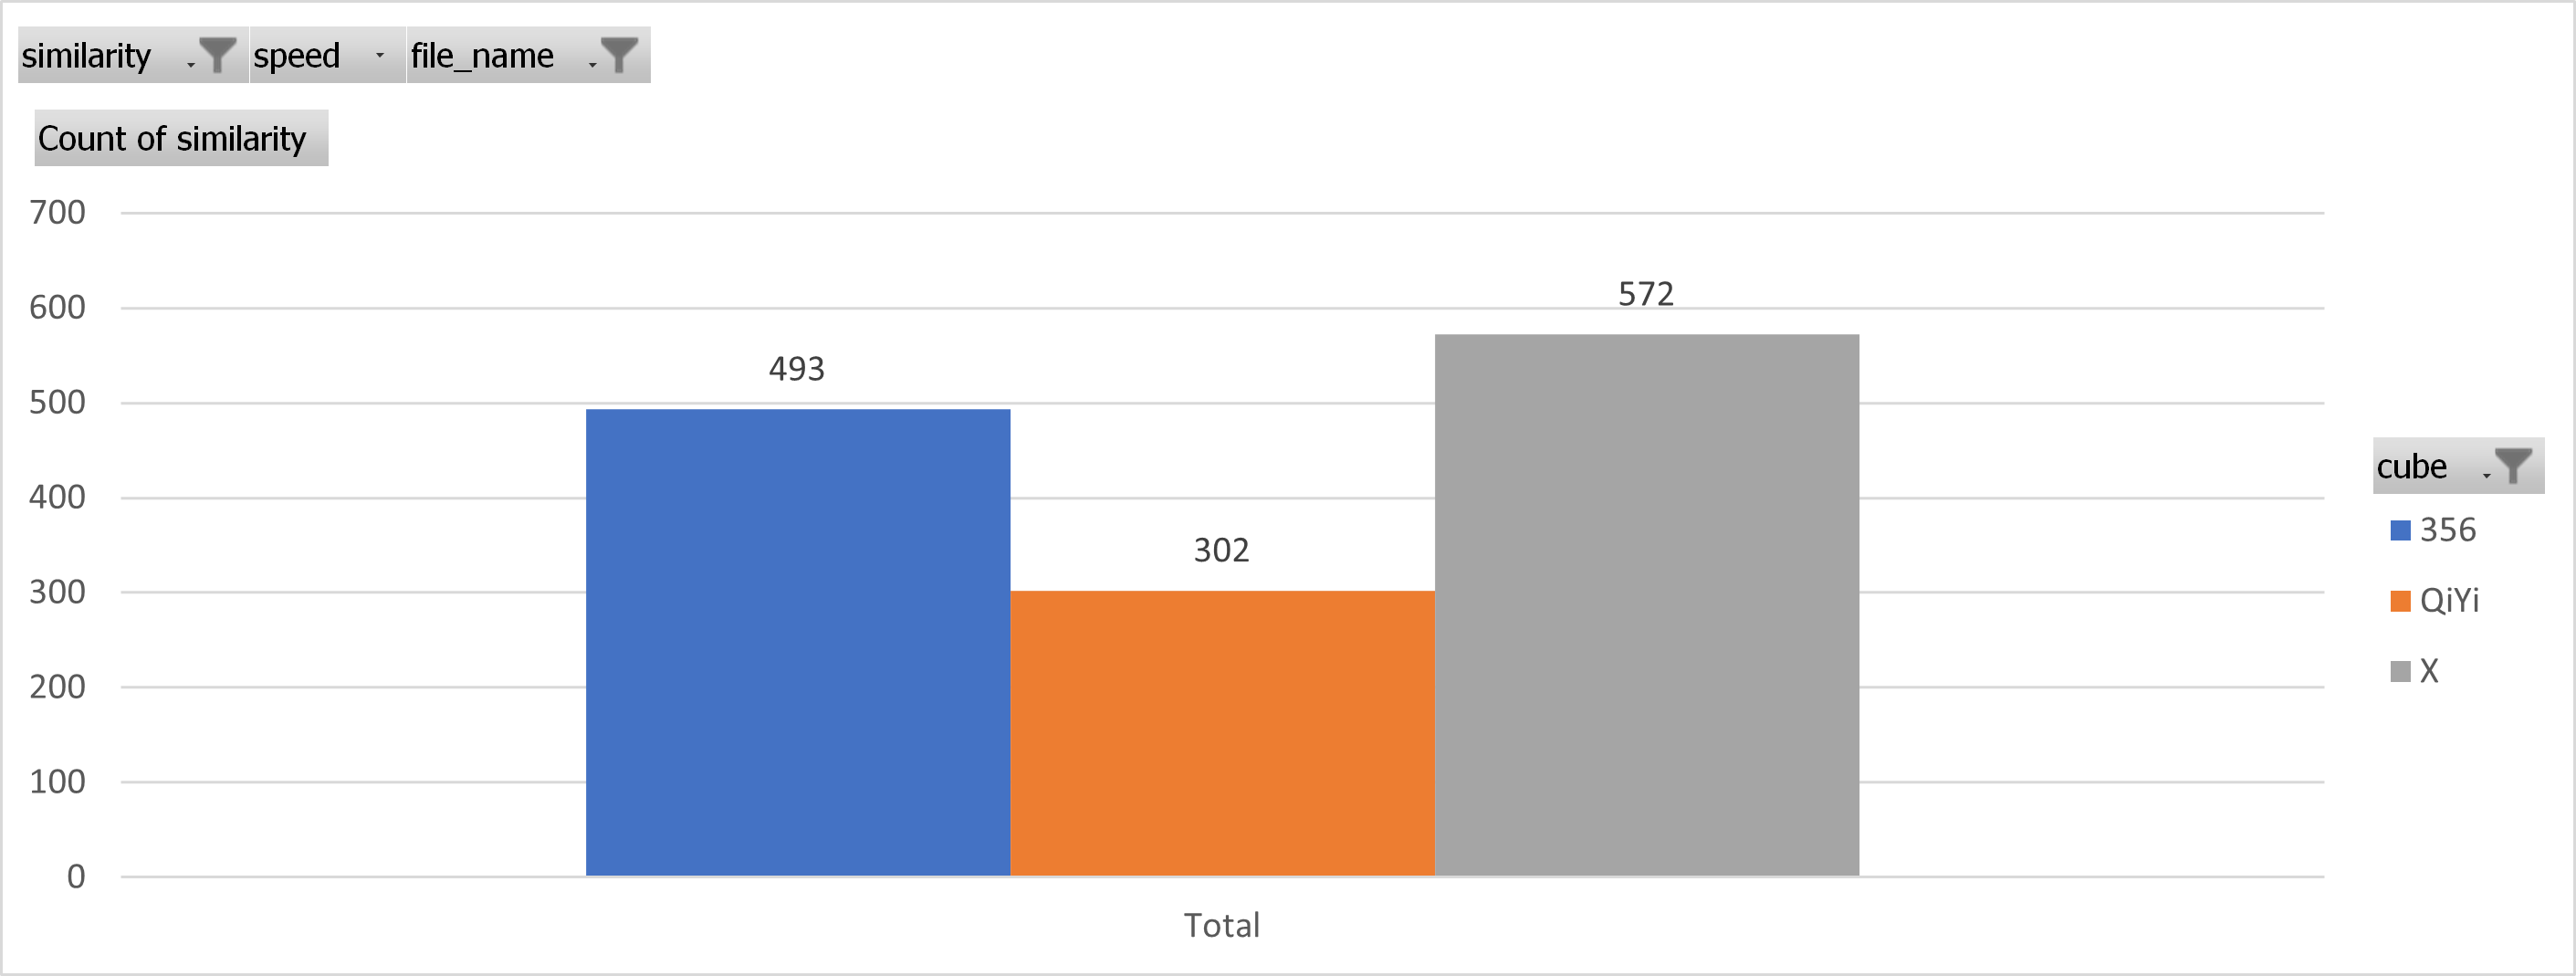
\includegraphics[width=\linewidth]{Figures/7 Evaluation/perfect_detections_by_cube.png}
    \vspace*{.1mm}
\end{subfigure}\\
\begin{subfigure}{\textwidth}
    \centering
    \caption{Total number of perfect detections at 2TPS}
    \label{fig:perfect-detections-by-cube-2tps}
    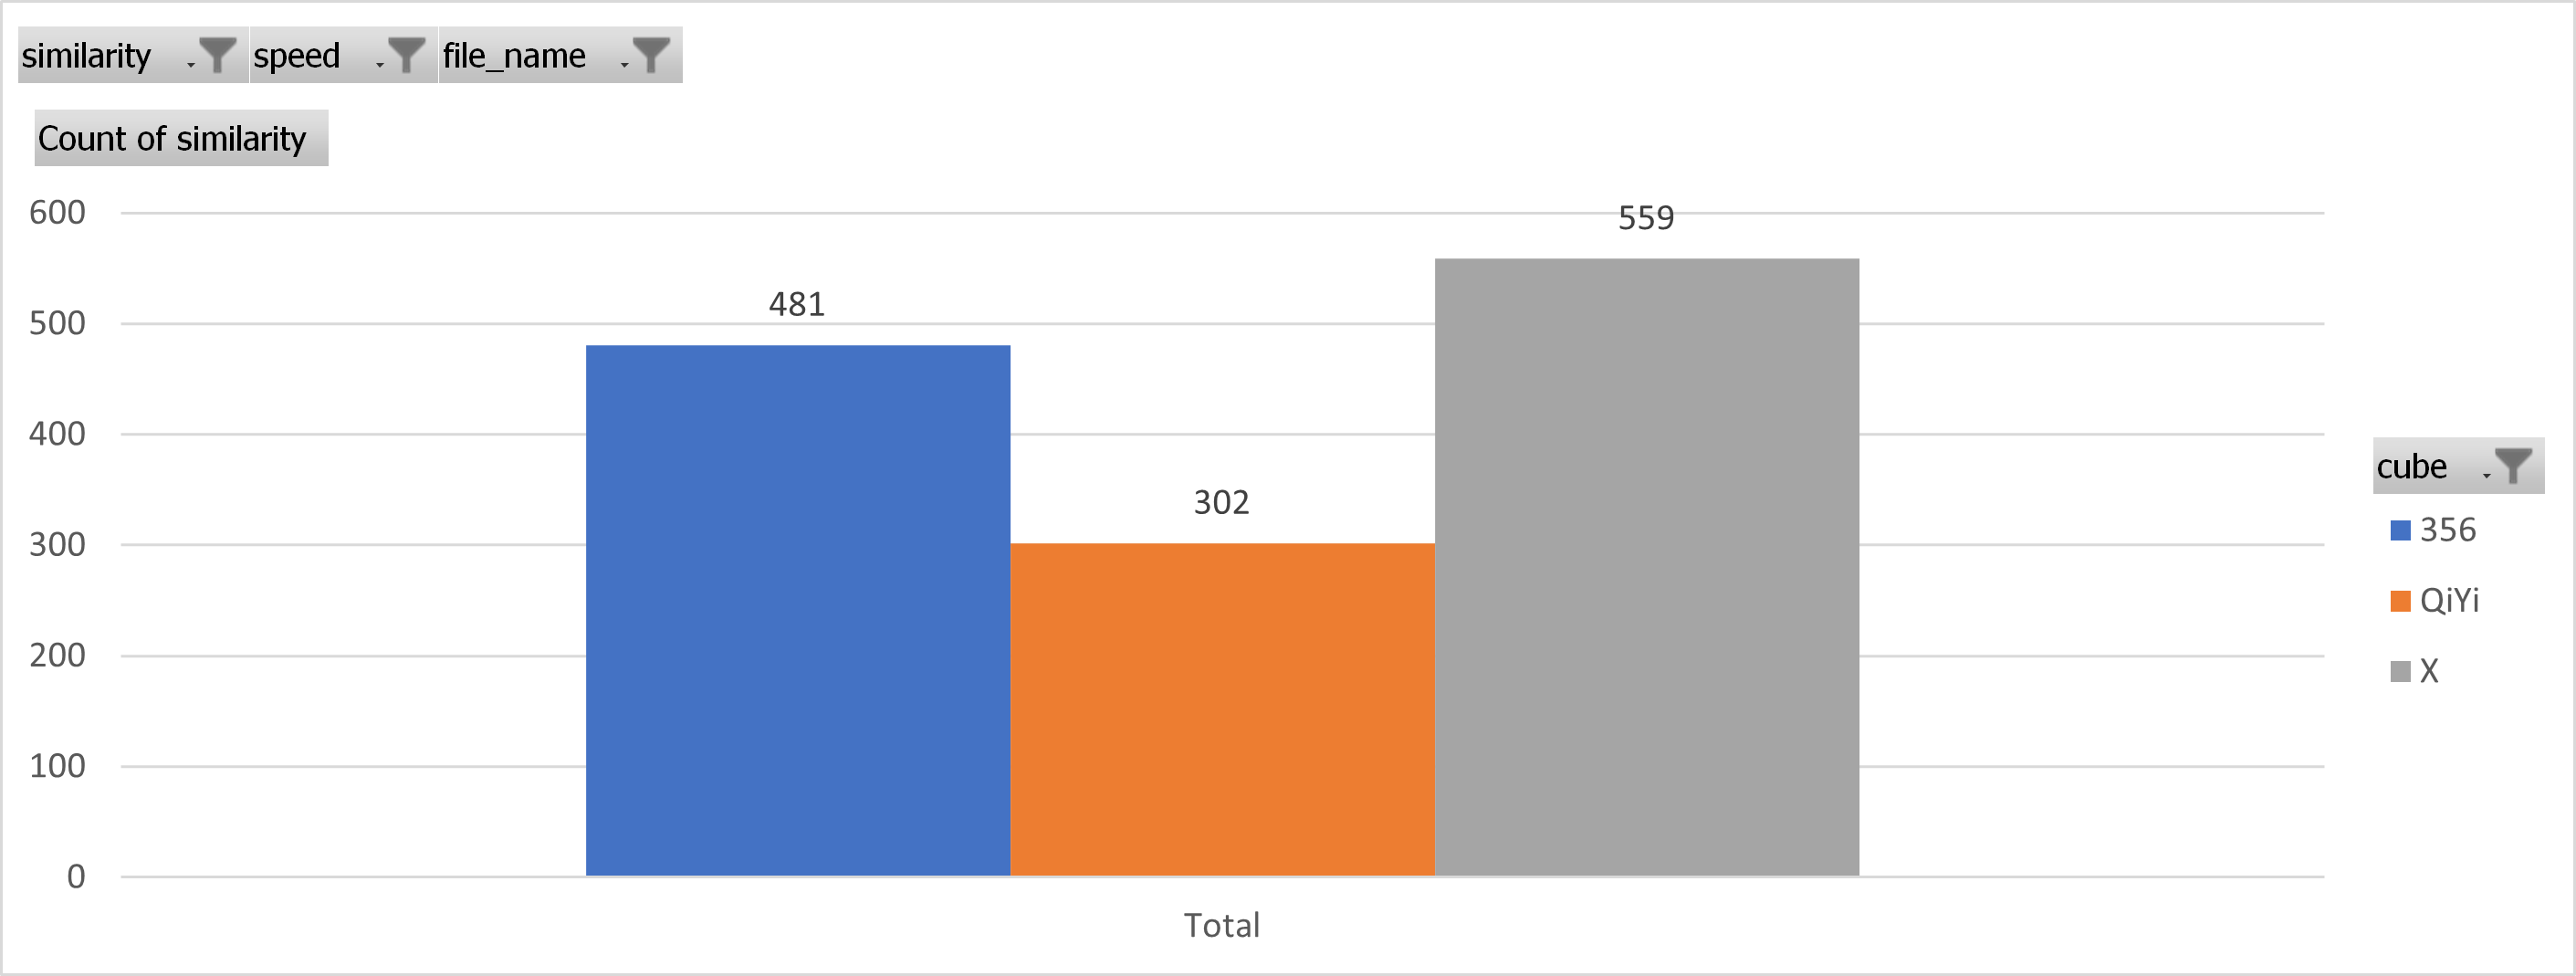
\includegraphics[width=\linewidth]{Figures/7 Evaluation/perfect_detections_by_cube_2tps.png}
    \vspace*{.1mm}
\end{subfigure}\\
\begin{subfigure}{\textwidth}
    \centering
    \caption{Total number of perfect detections at 5TPS}
    \label{fig:perfect-detections-by-cube-5tps}
    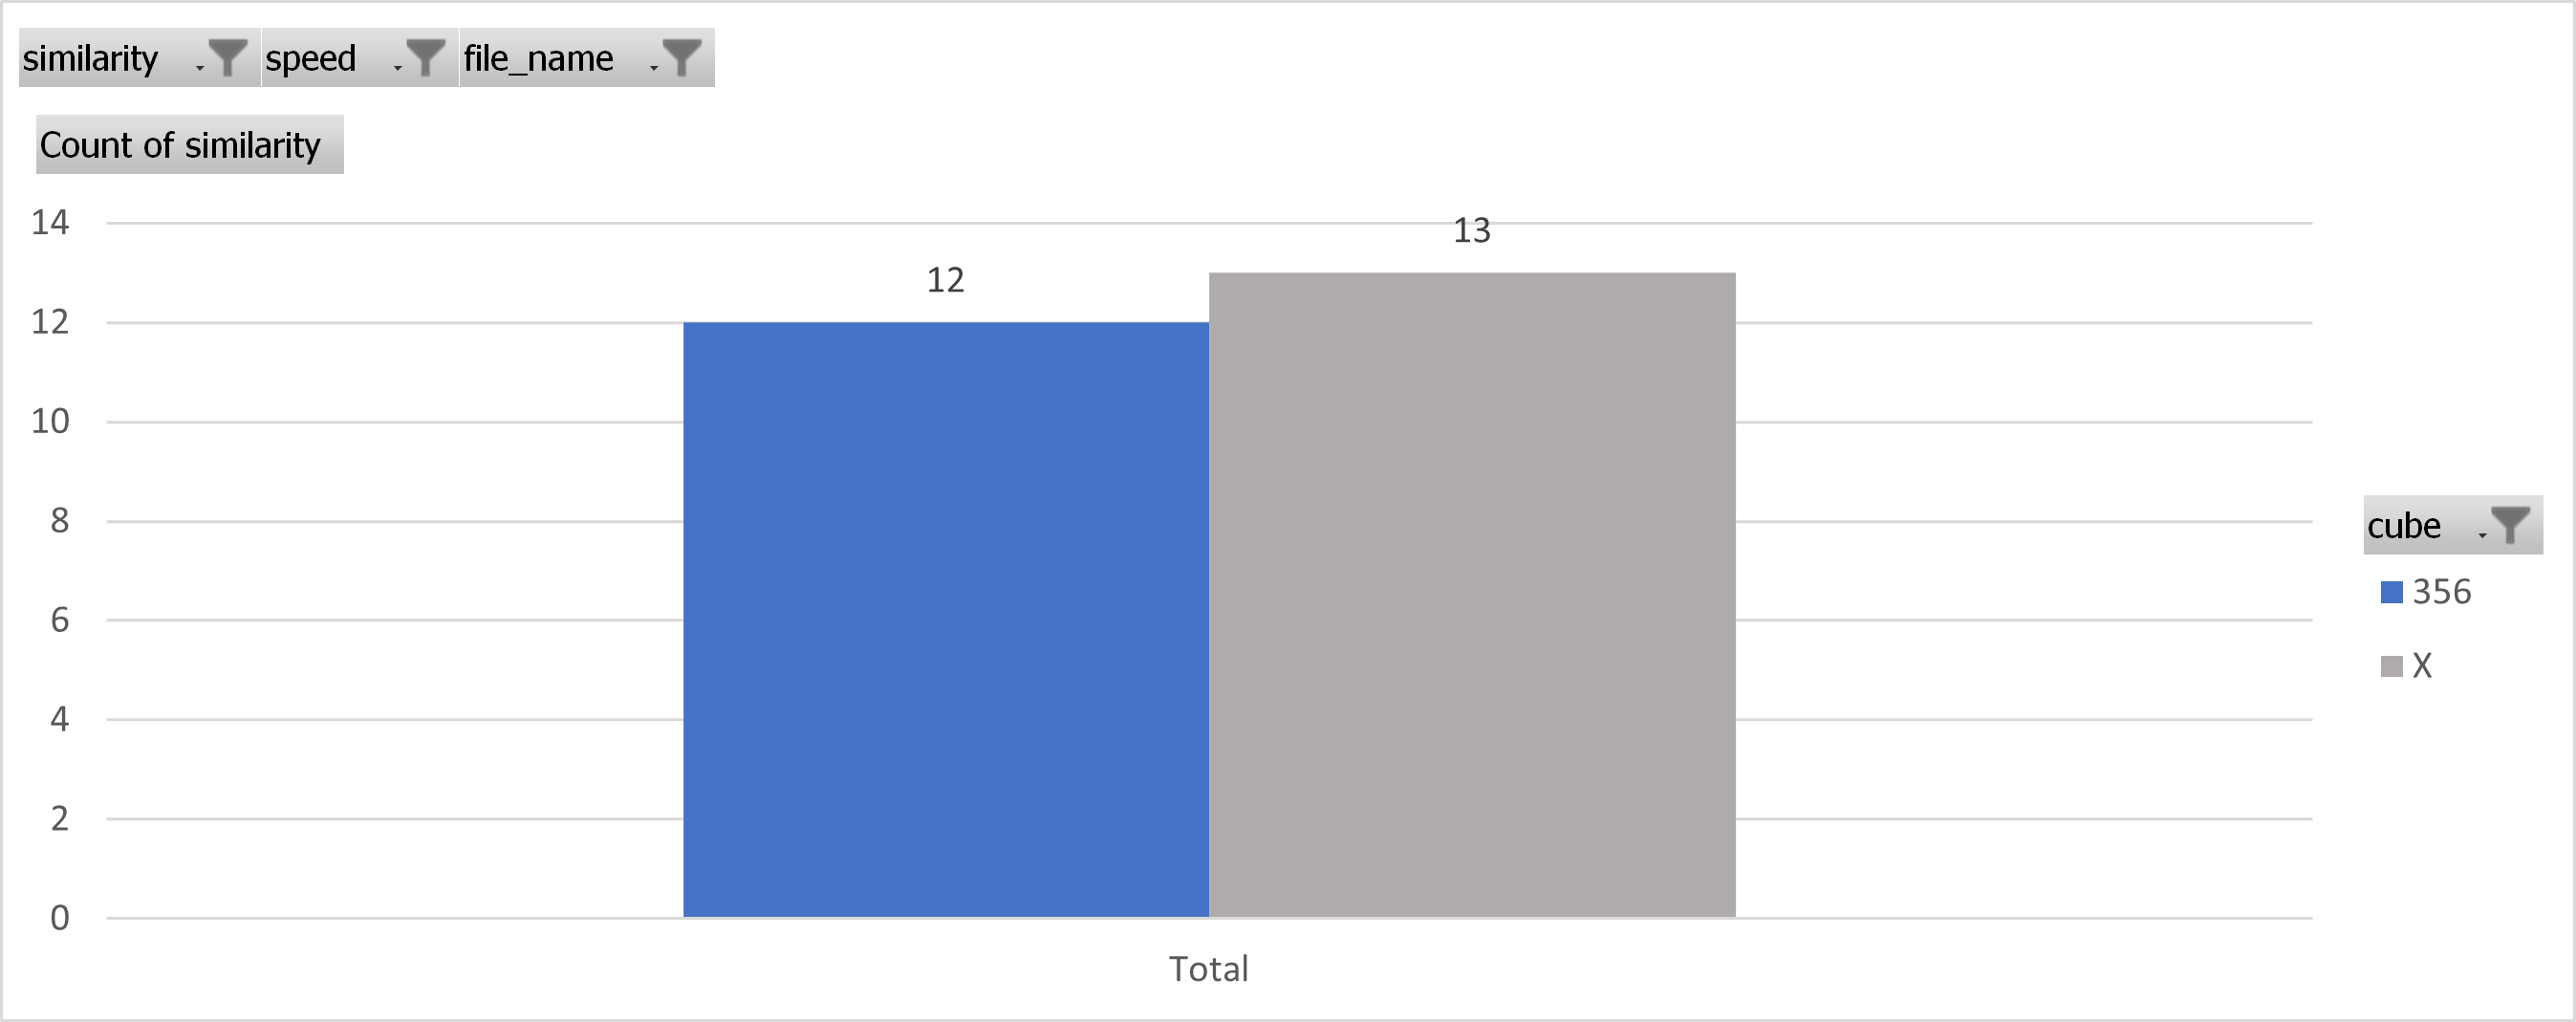
\includegraphics[width=\linewidth]{Figures/7 Evaluation/perfect_detections_by_cube_5tps.png}
    \vspace*{.1mm}
\end{subfigure}\\
\end{figure}

Figure \ref{fig:perfect-detections-by-cube} shows the total number of
perfect move sequence decodings broken down by cube type and simulated
turn speed. As expected, there were far fewer perfect detections at the
higher simulated turn speed compared to the lower simulated turn speed,
with the loud QiYi even failing to register a single perfect detection
at the higher turn speed. However, it was the normal noise Gans XS, not
the quiet Gans 356 that achieved the most perfect detections. This is a
peculiar result since Figure \ref{fig:signal-to-noise-ratio} shows that
the Gans XS is louder across a wider frequency spectrum than the Gans
356.

\subsection{Influence of the Standard Deviation Threshold}
\label{subsec:influence-stdv-threshold}

The standard deviation threshold was one piece of the threshold
calculation used to filter out background noise (see Section
\ref{subsec:fine-tuning-threshold}). Since frequency peaks tend to be
statistical outliers, higher thresholds were expected to filter out
more background noise, thus providing higher detection accuracy, so
long as the thresholds were not so high as to exclude the peaks
themselves.

Figure \ref{fig:influence-stdv-threshold-perfect} shows the total number of
perfect move sequence decodings broken down by the standard deviation
threshold. Contrary to the expectations, the slightly sinusoidal results show that lower thresholds generally corresponded to slightly better chances of achieving a perfect detection than higher thresholds.

However, Figures \ref{fig:influence-stdv-threshold-average-2tps} and
\ref{fig:influence-stdv-threshold-average-5tps} suggest that, overall,
a higher standard deviation threshold typically corresponds to a higher
average detection accuracy across all variations of the other parameters in
this experiment. Of particular interest is the continuous improvement
in detection accuracy experienced by the noisy QiYi Qimeng as the
standard deviation threshold increased, particularly for the 5TPS audio
sequences where it achieved a higher average accuracy than either of
its less noisy counterparts.

\begin{figure}
    \caption{Influence of Standard Deviation Threshold on Accuracy}
    \label{fig:influence-stdv-threshold}
    \begin{subfigure}{\textwidth}
        \centering
        \caption{Perfect Detections by Standard Deviation Threshold}
        \label{fig:influence-stdv-threshold-perfect}
        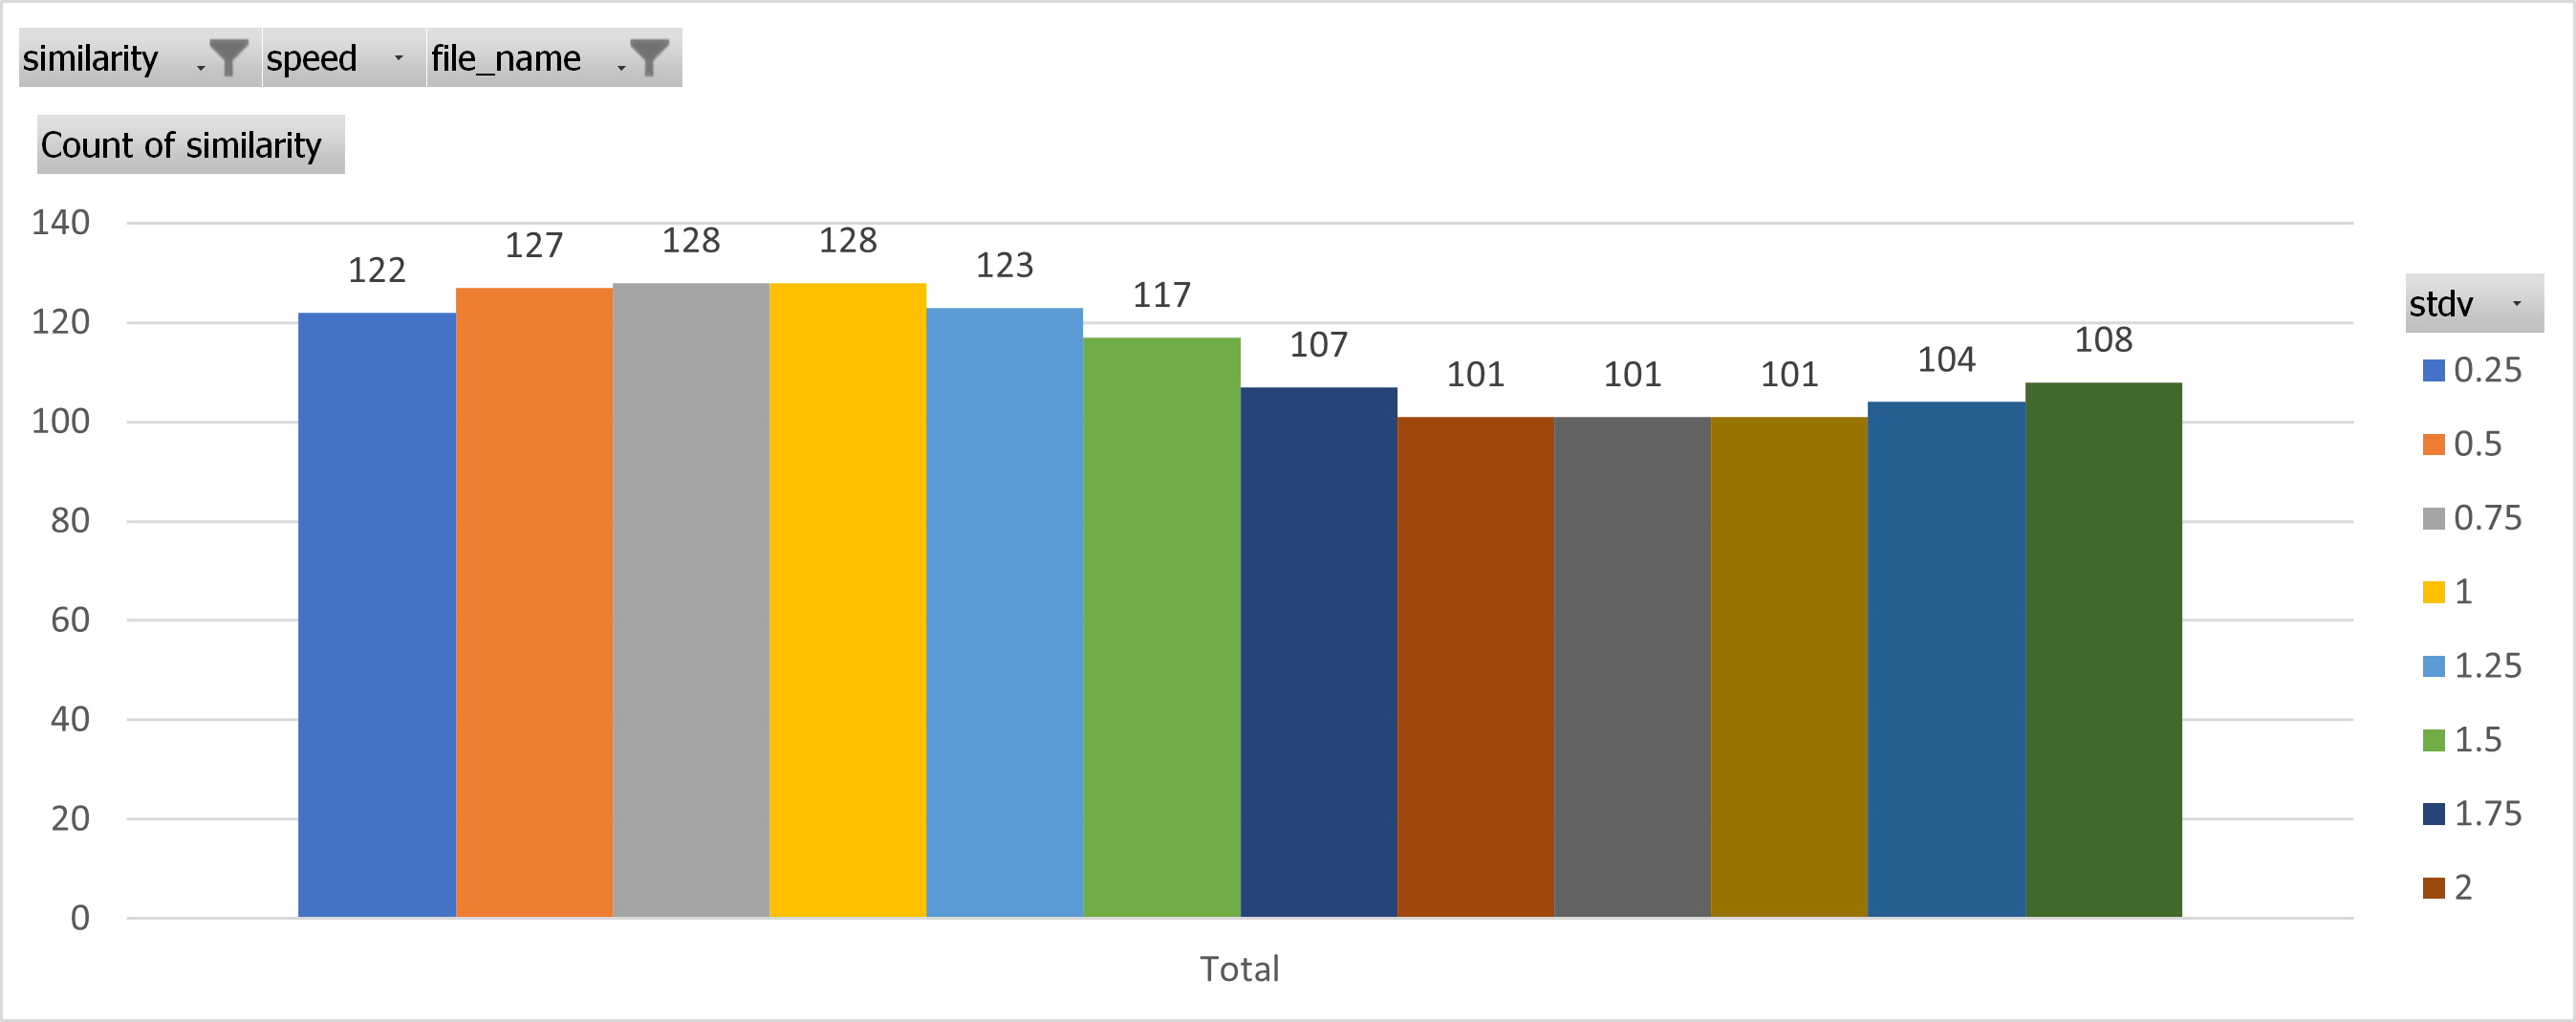
\includegraphics[width=\linewidth]{Figures/7 Evaluation/perfect_detections_by_stdv.png}
        \vspace*{.1mm}
    \end{subfigure}\\
    \begin{subfigure}{\textwidth}
        \centering
        \caption{Average Accuracy by Standard Deviation Threshold at 2 TPS}
        \label{fig:influence-stdv-threshold-average-2tps}
        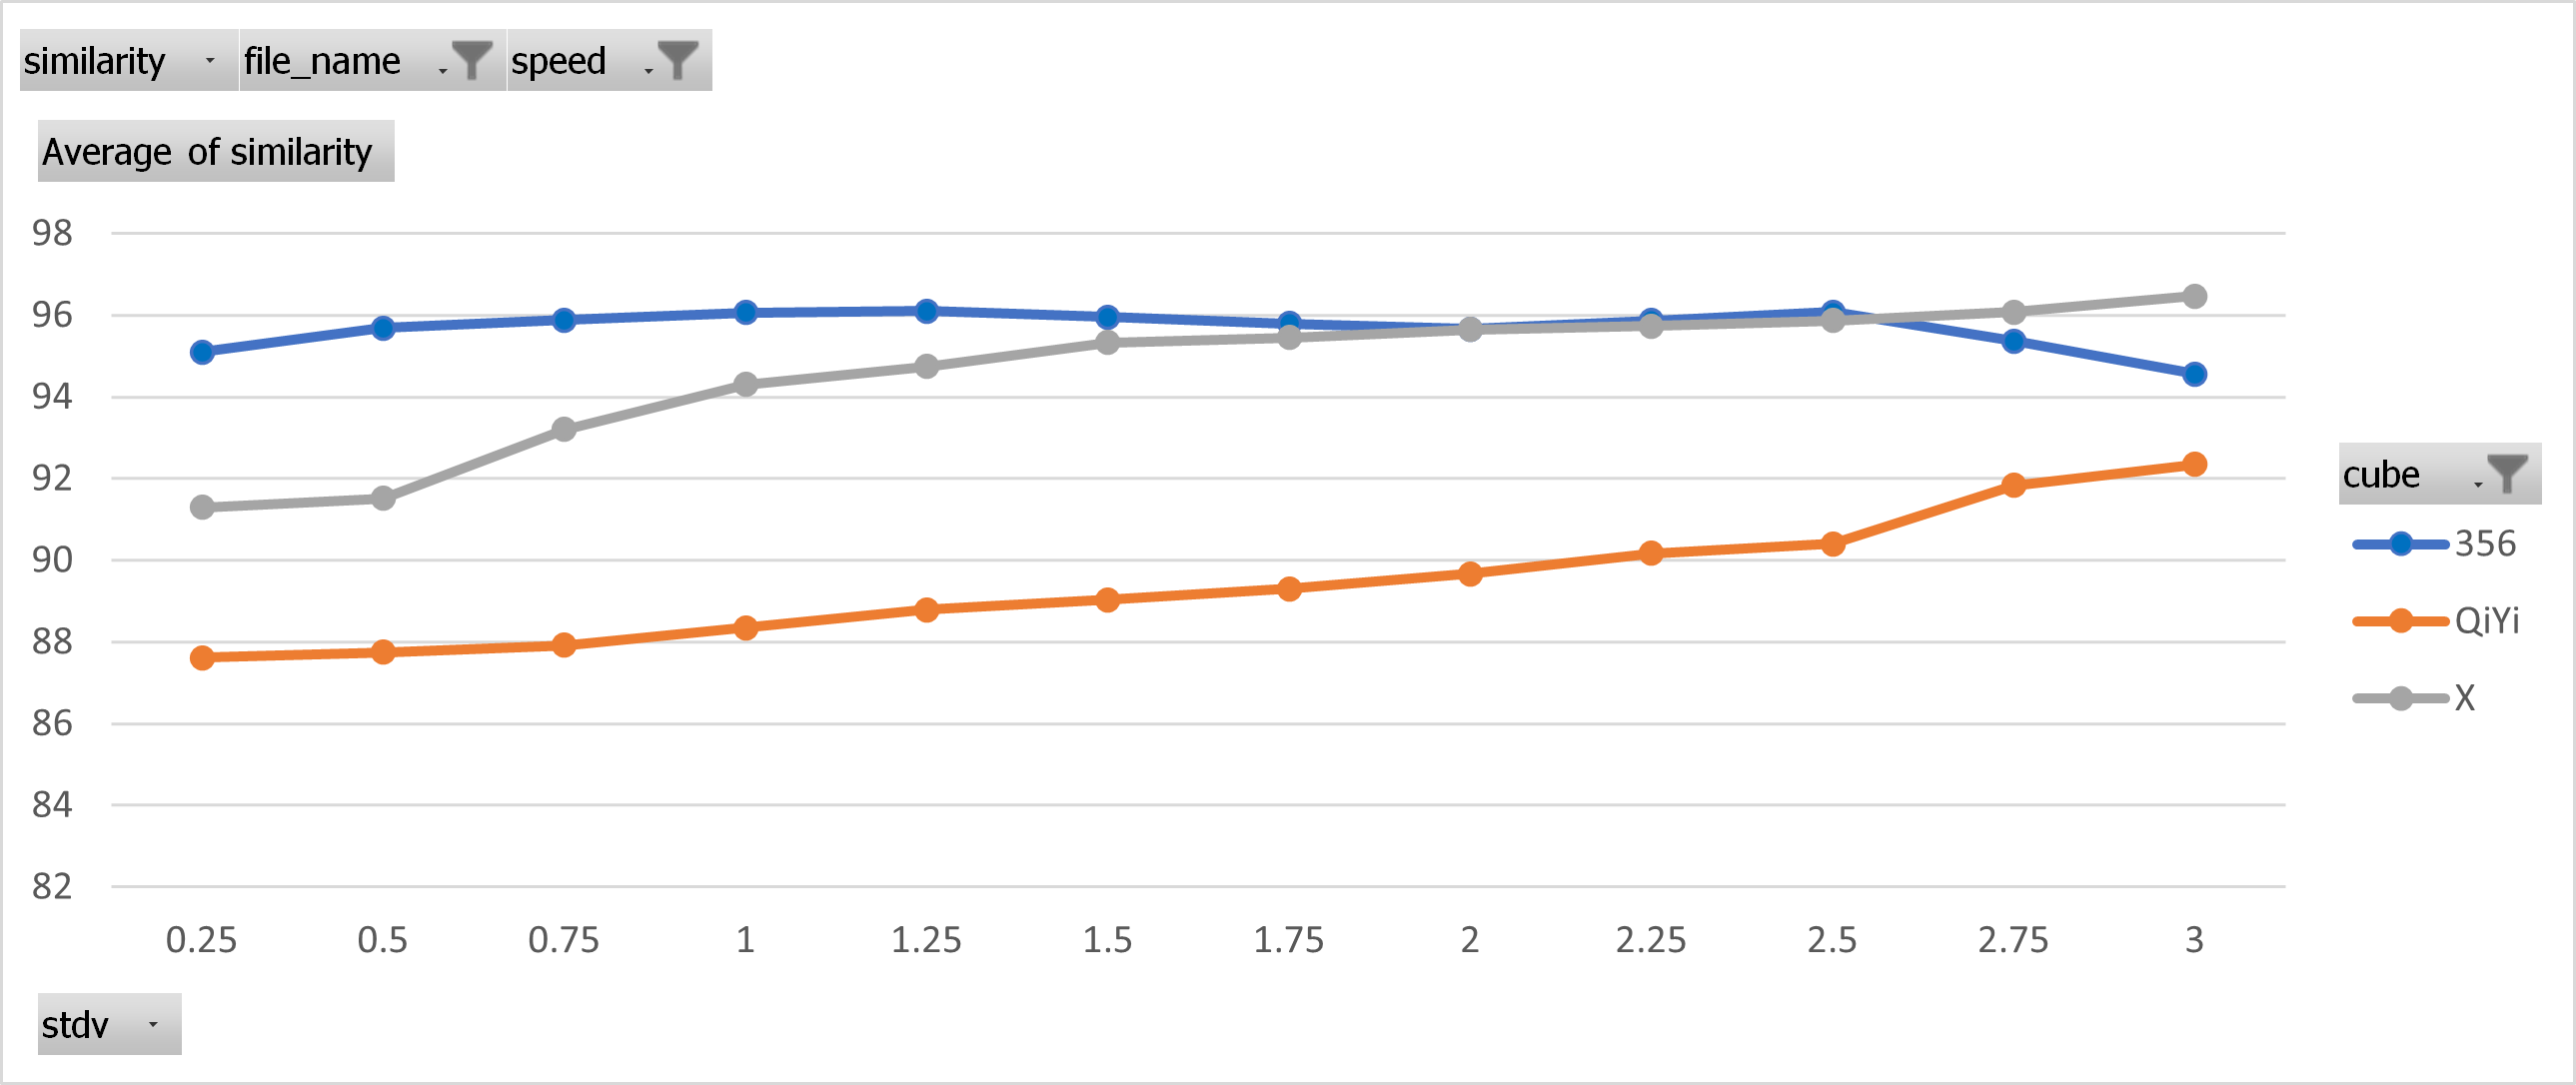
\includegraphics[width=\linewidth]{Figures/7 Evaluation/similarity_by_stdv_2tps.png}
        \vspace*{.1mm}
    \end{subfigure}\\
    \begin{subfigure}{\textwidth}
        \centering
        \caption{Average Accuracy by Standard Deviation Threshold at 5 TPS}
        \label{fig:influence-stdv-threshold-average-5tps}
        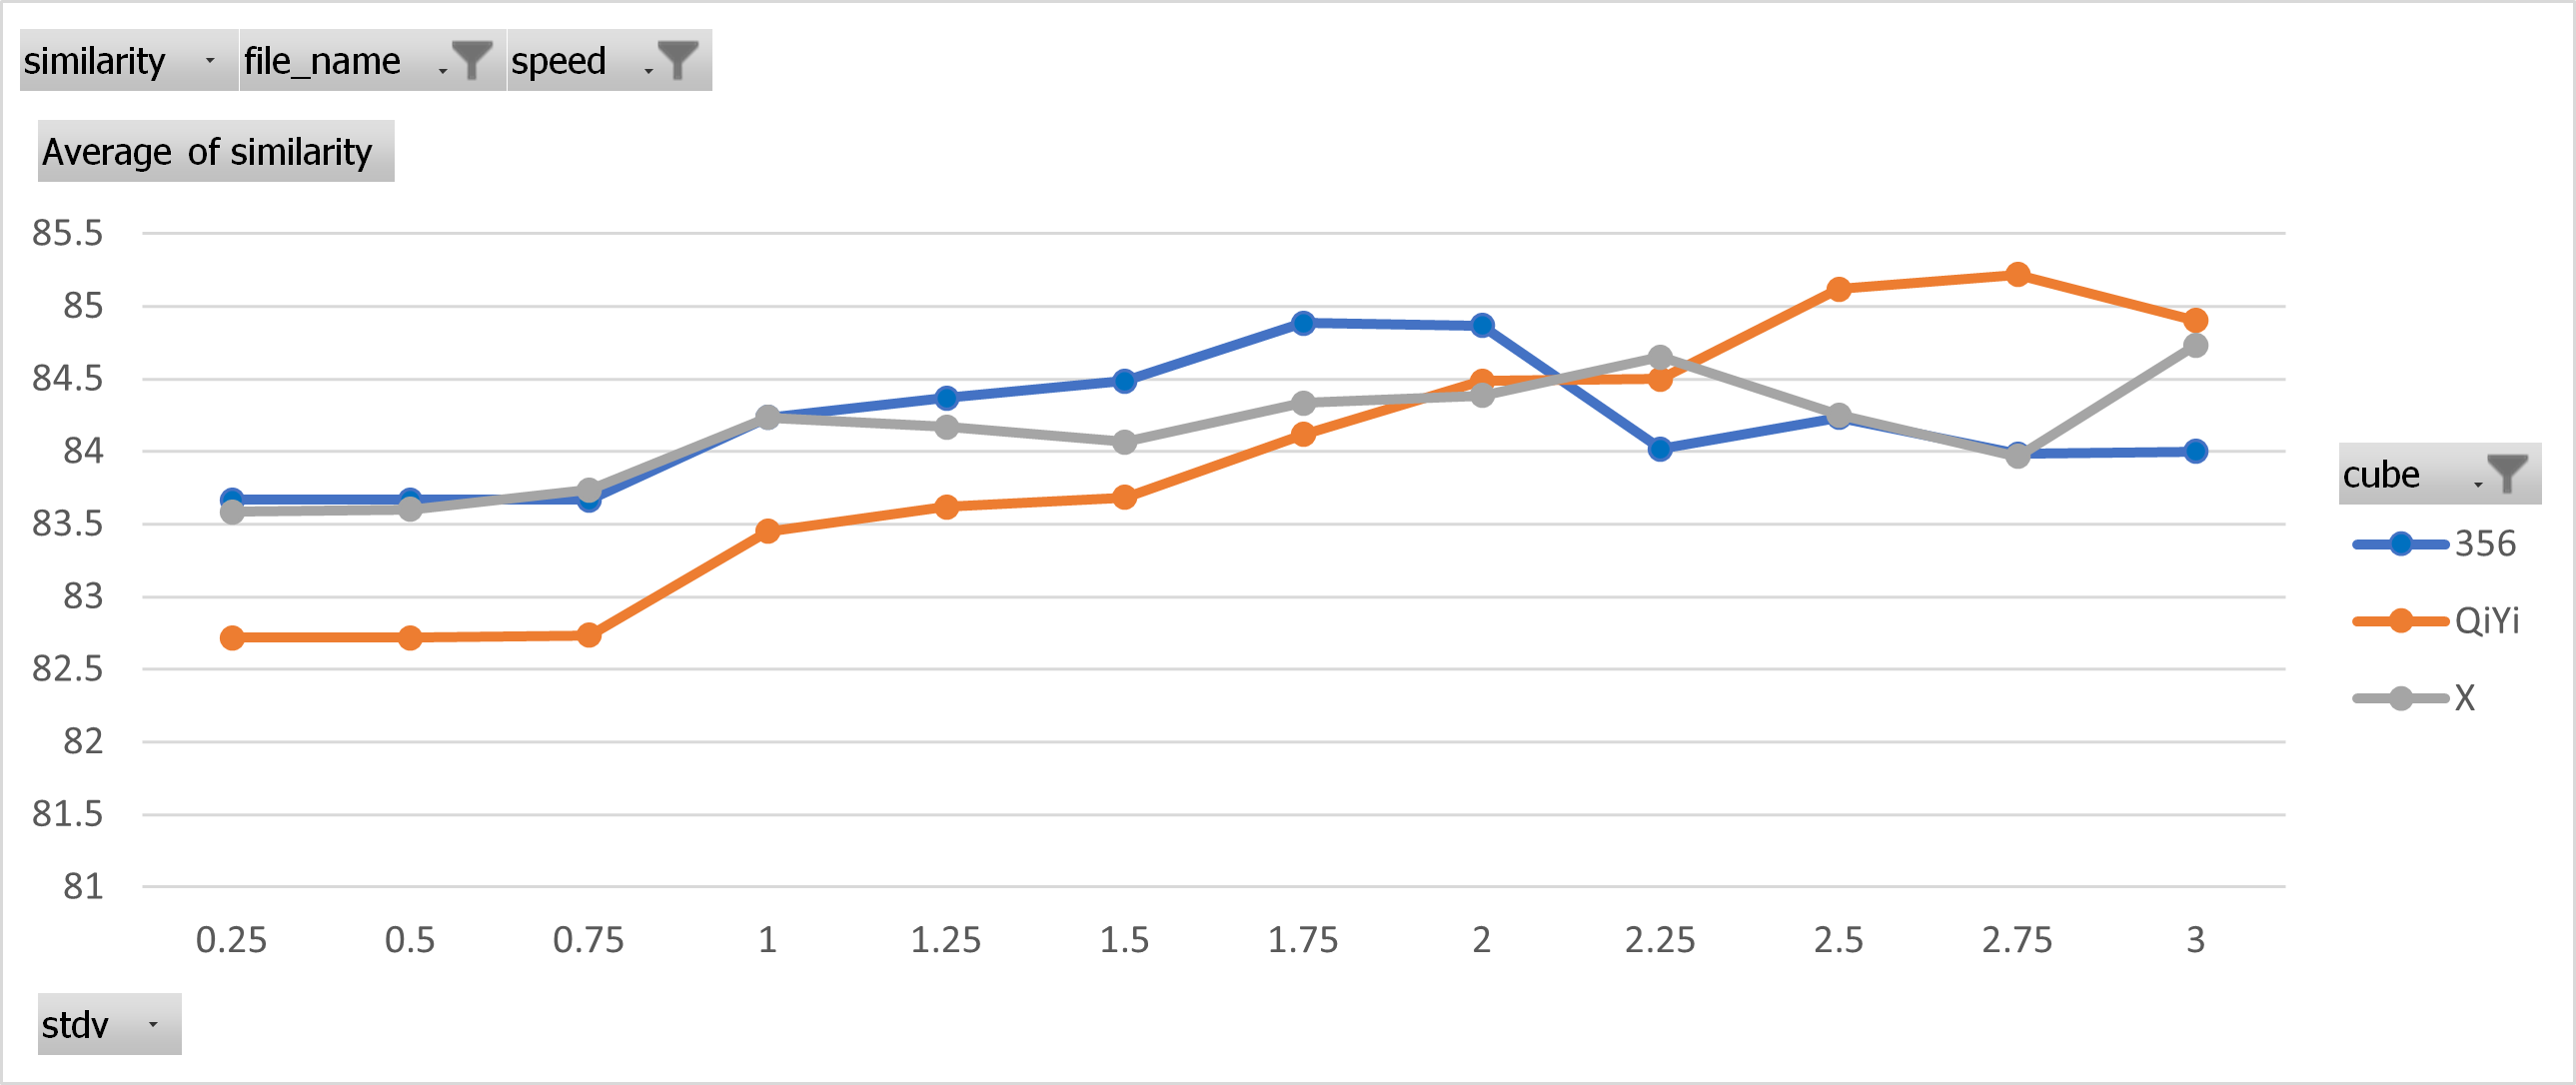
\includegraphics[width=\linewidth]{Figures/7 Evaluation/similarity_by_stdv_5tps.png}
        \vspace*{.1mm}
    \end{subfigure}\\
\end{figure}

\subsection{Influence of Minimum Threshold}
\label{subsec:influence-alt-min}

The minimum threshold was the second component in the threshold
calculation discussed in Section \ref{subsec:fine-tuning-threshold},
used primarily to filter out background noise during the quiet signal
period between face turns. Similar to the standard deviation threshold,
higher minimum thresholds were expected to yield higher detection
accuracies, particularly for noisy cubes.

Interestingly, the minimum threshold performed similarly to the
standard deviation threshold in regard to its correlation with perfect
move sequence detections (Figure
\ref{fig:perfect-detections-by-alt-min-total}). However, in contrast to
the standard deviation threshold, the minimum threshold corresponded to
far less variation in the average accuracy, though accuracy did trend
upwards as the minimum threshold increased.

\begin{figure}
    \caption{Perfect Detections by Minimum Threshold}
    \label{fig:influence-alt-min}
    \begin{subfigure}{\textwidth}
        \centering
        \caption{Total number of perfect detections}
        \label{fig:perfect-detections-by-alt-min-total}
        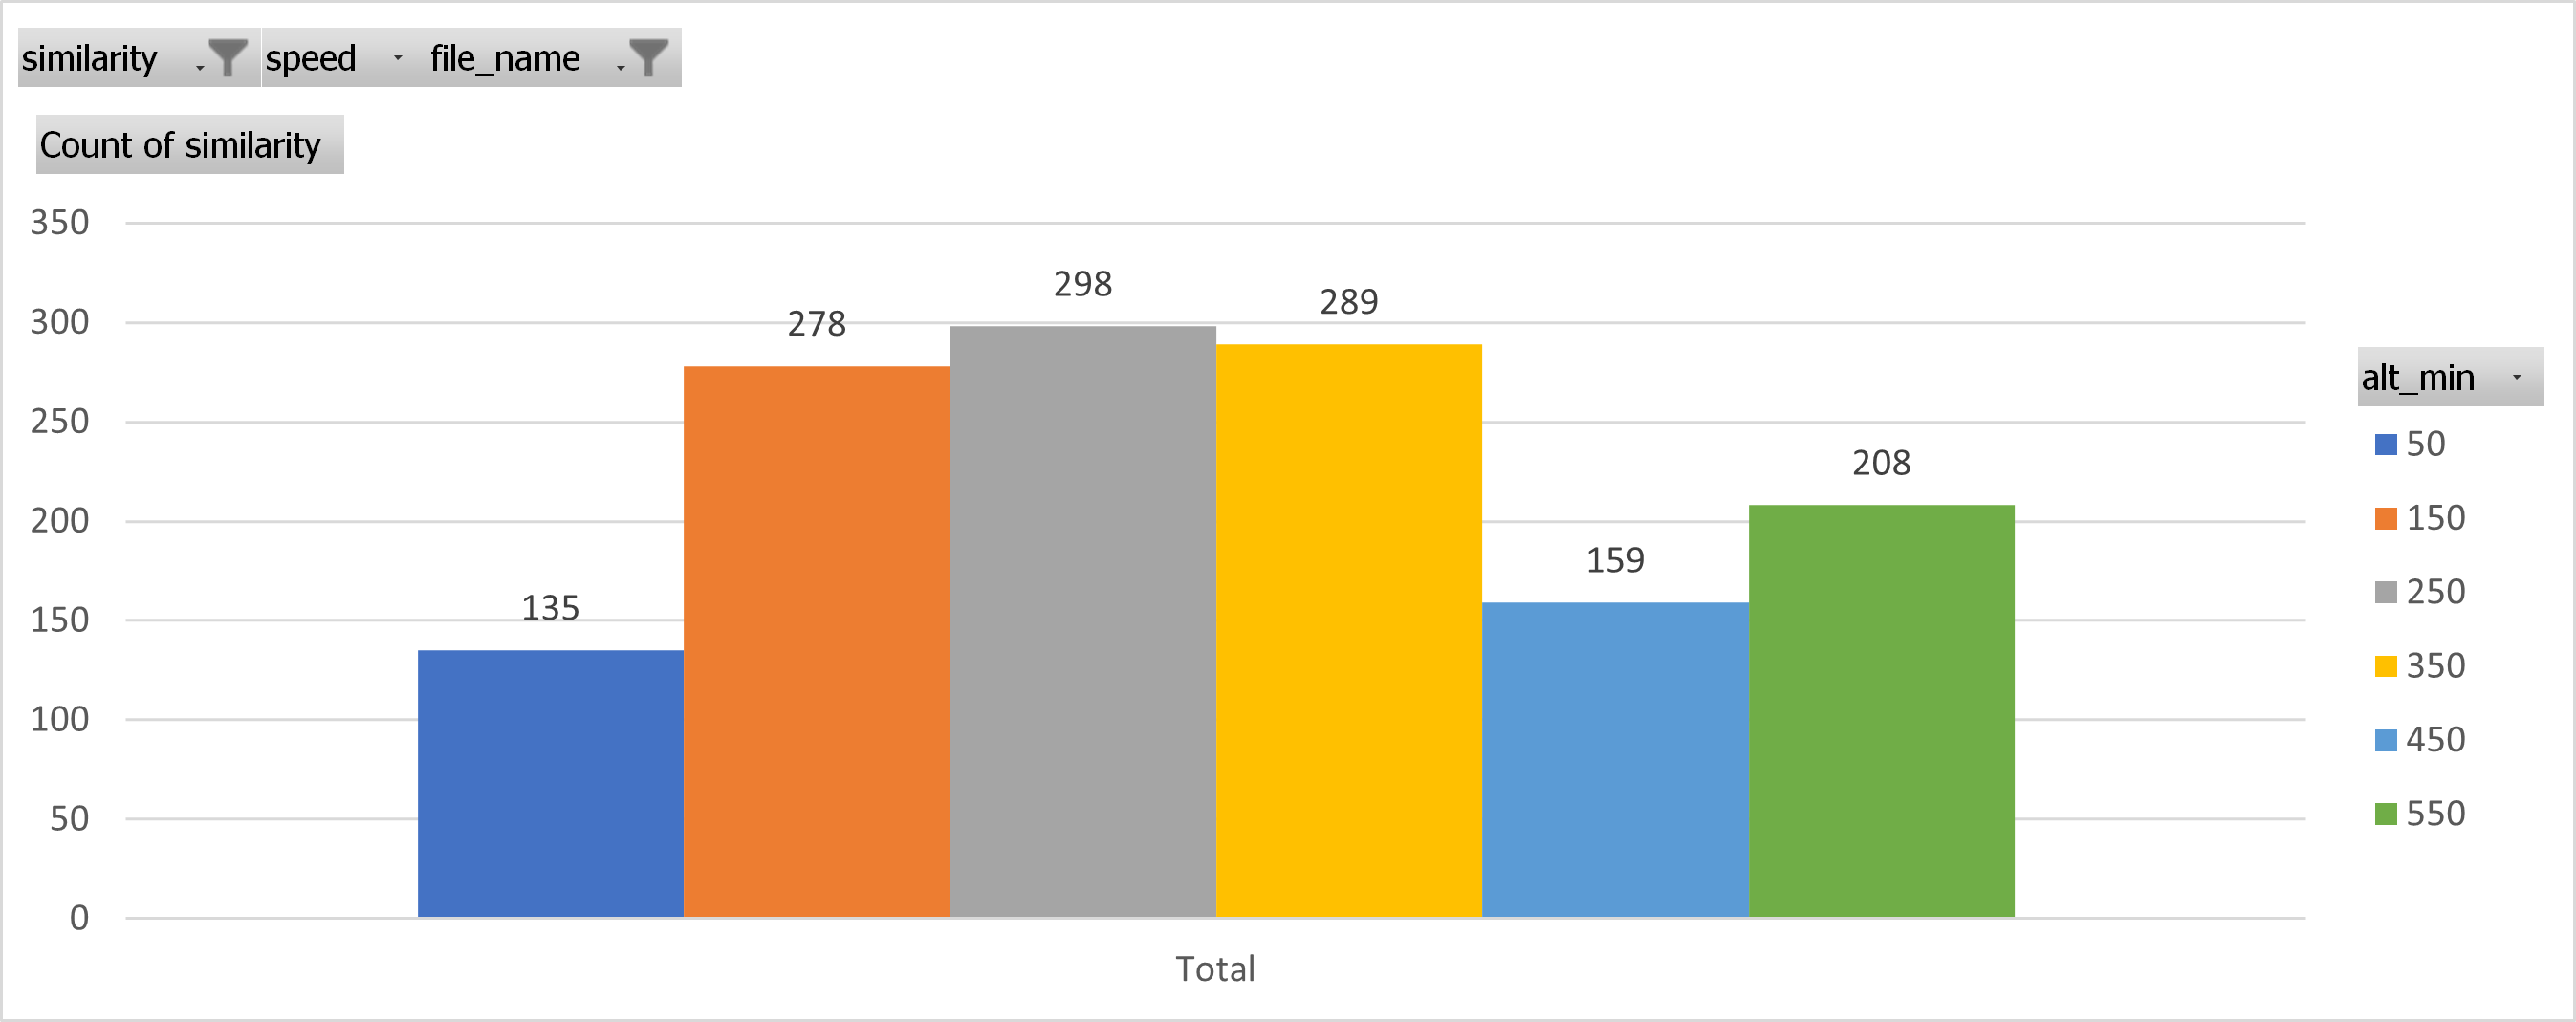
\includegraphics[width=\linewidth]{Figures/7 Evaluation/perfect_detections_by_alt_min.png}
        \vspace*{.1mm}
    \end{subfigure}\\
    \begin{subfigure}{\textwidth}
        \centering
        \caption{Average Accuracy by Minimum Threshold at 2 TPS}
        \label{fig:influence-alt-min-average-2tps}
        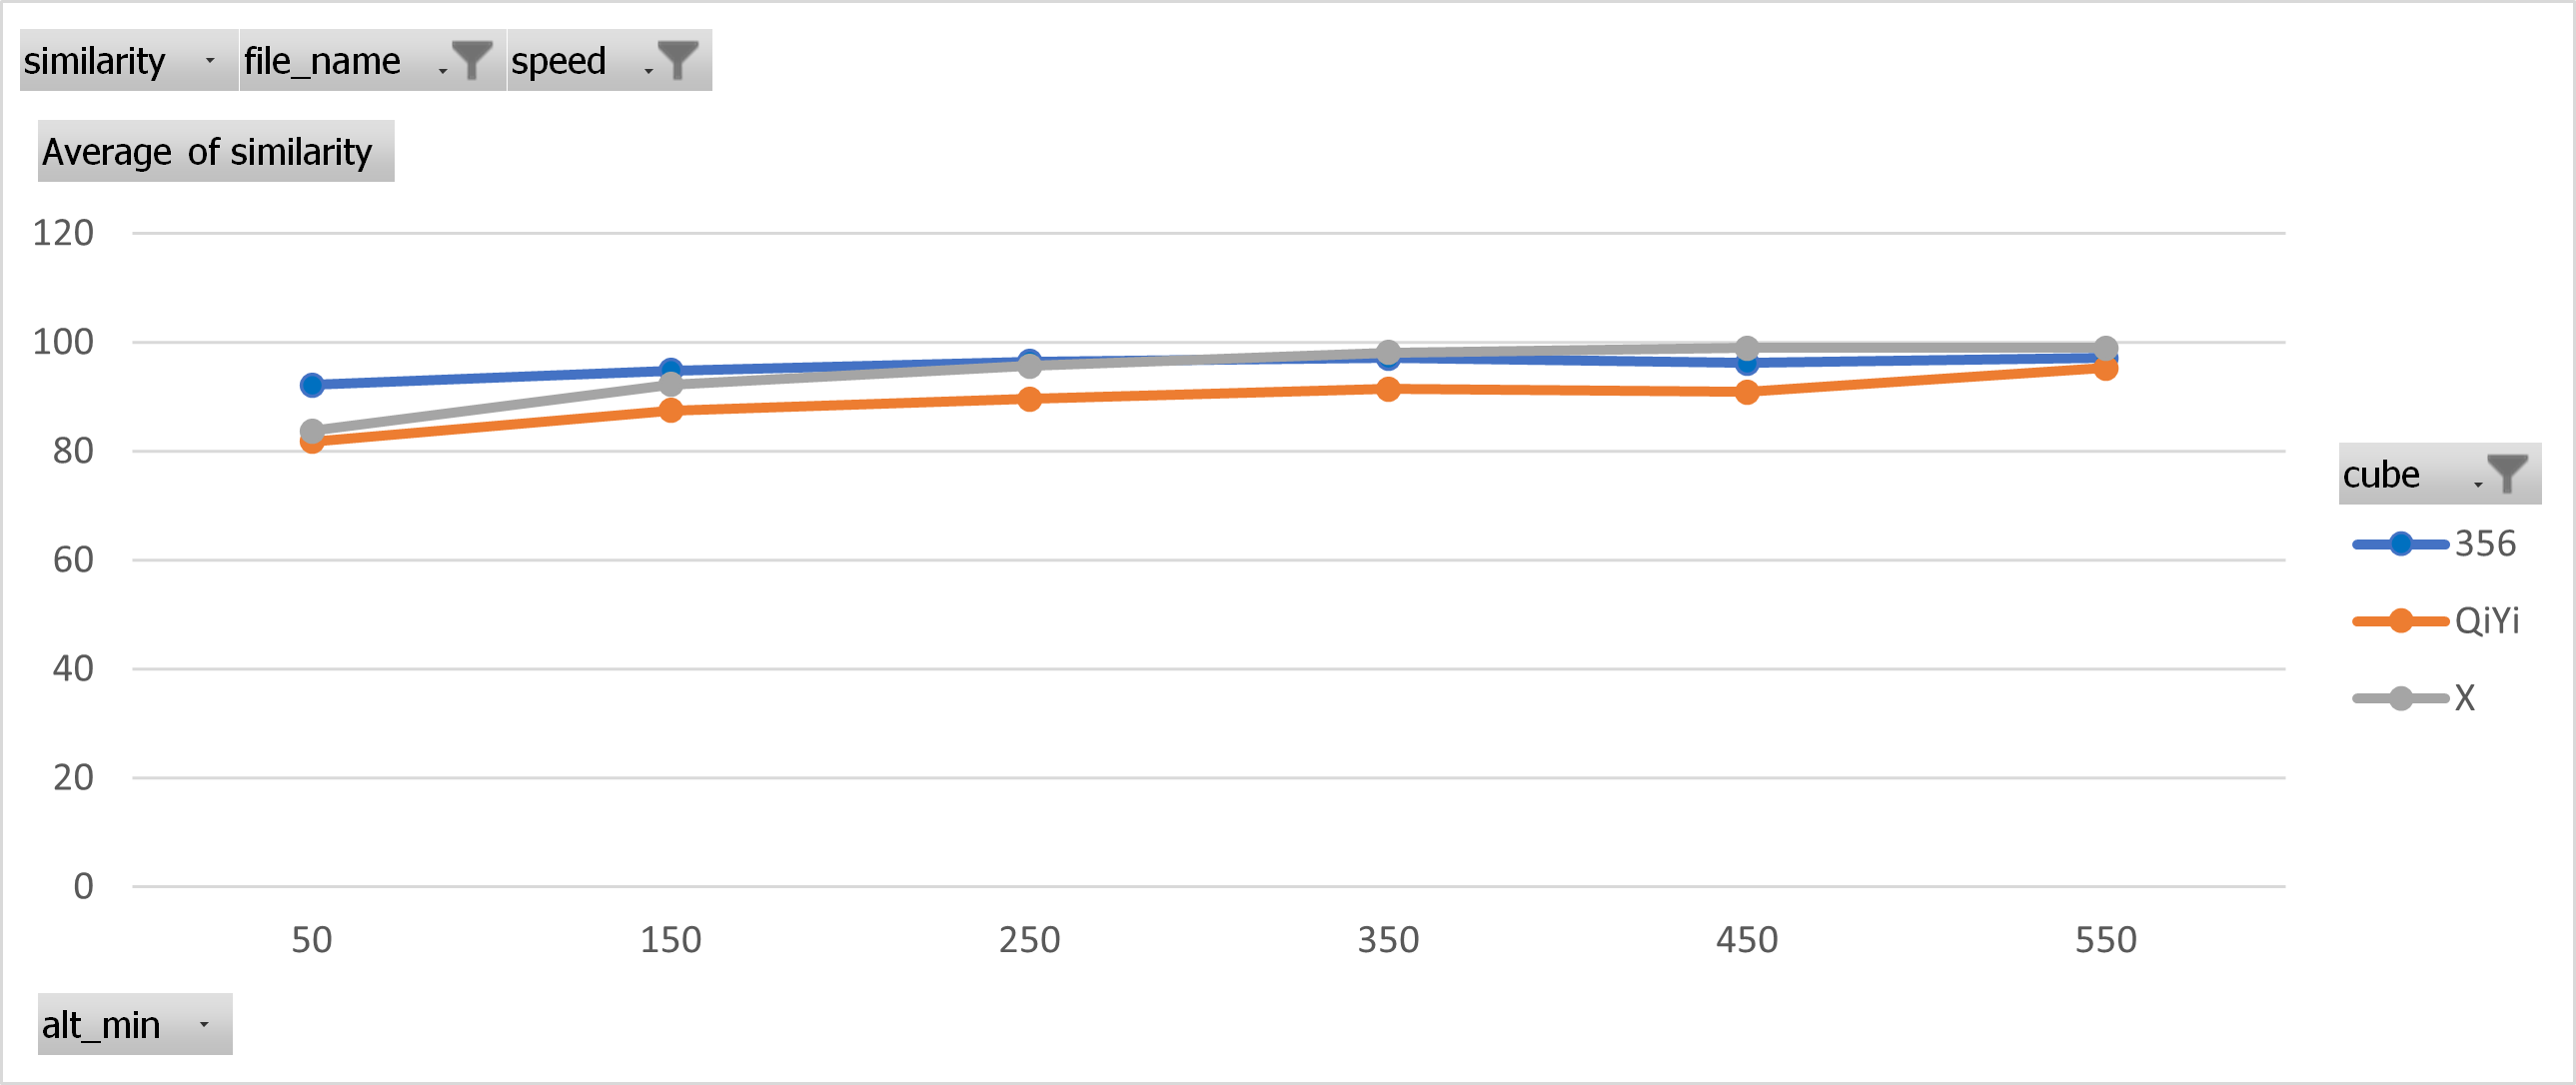
\includegraphics[width=\linewidth]{Figures/7 Evaluation/similarity_by_alt_min_2tps.png}
        \vspace*{.1mm}
    \end{subfigure}\\
    \begin{subfigure}{\textwidth}
        \centering
        \caption{Average Accuracy by Minimum Threshold at 5 TPS}
        \label{fig:influence-alt-min-average-5tps}
        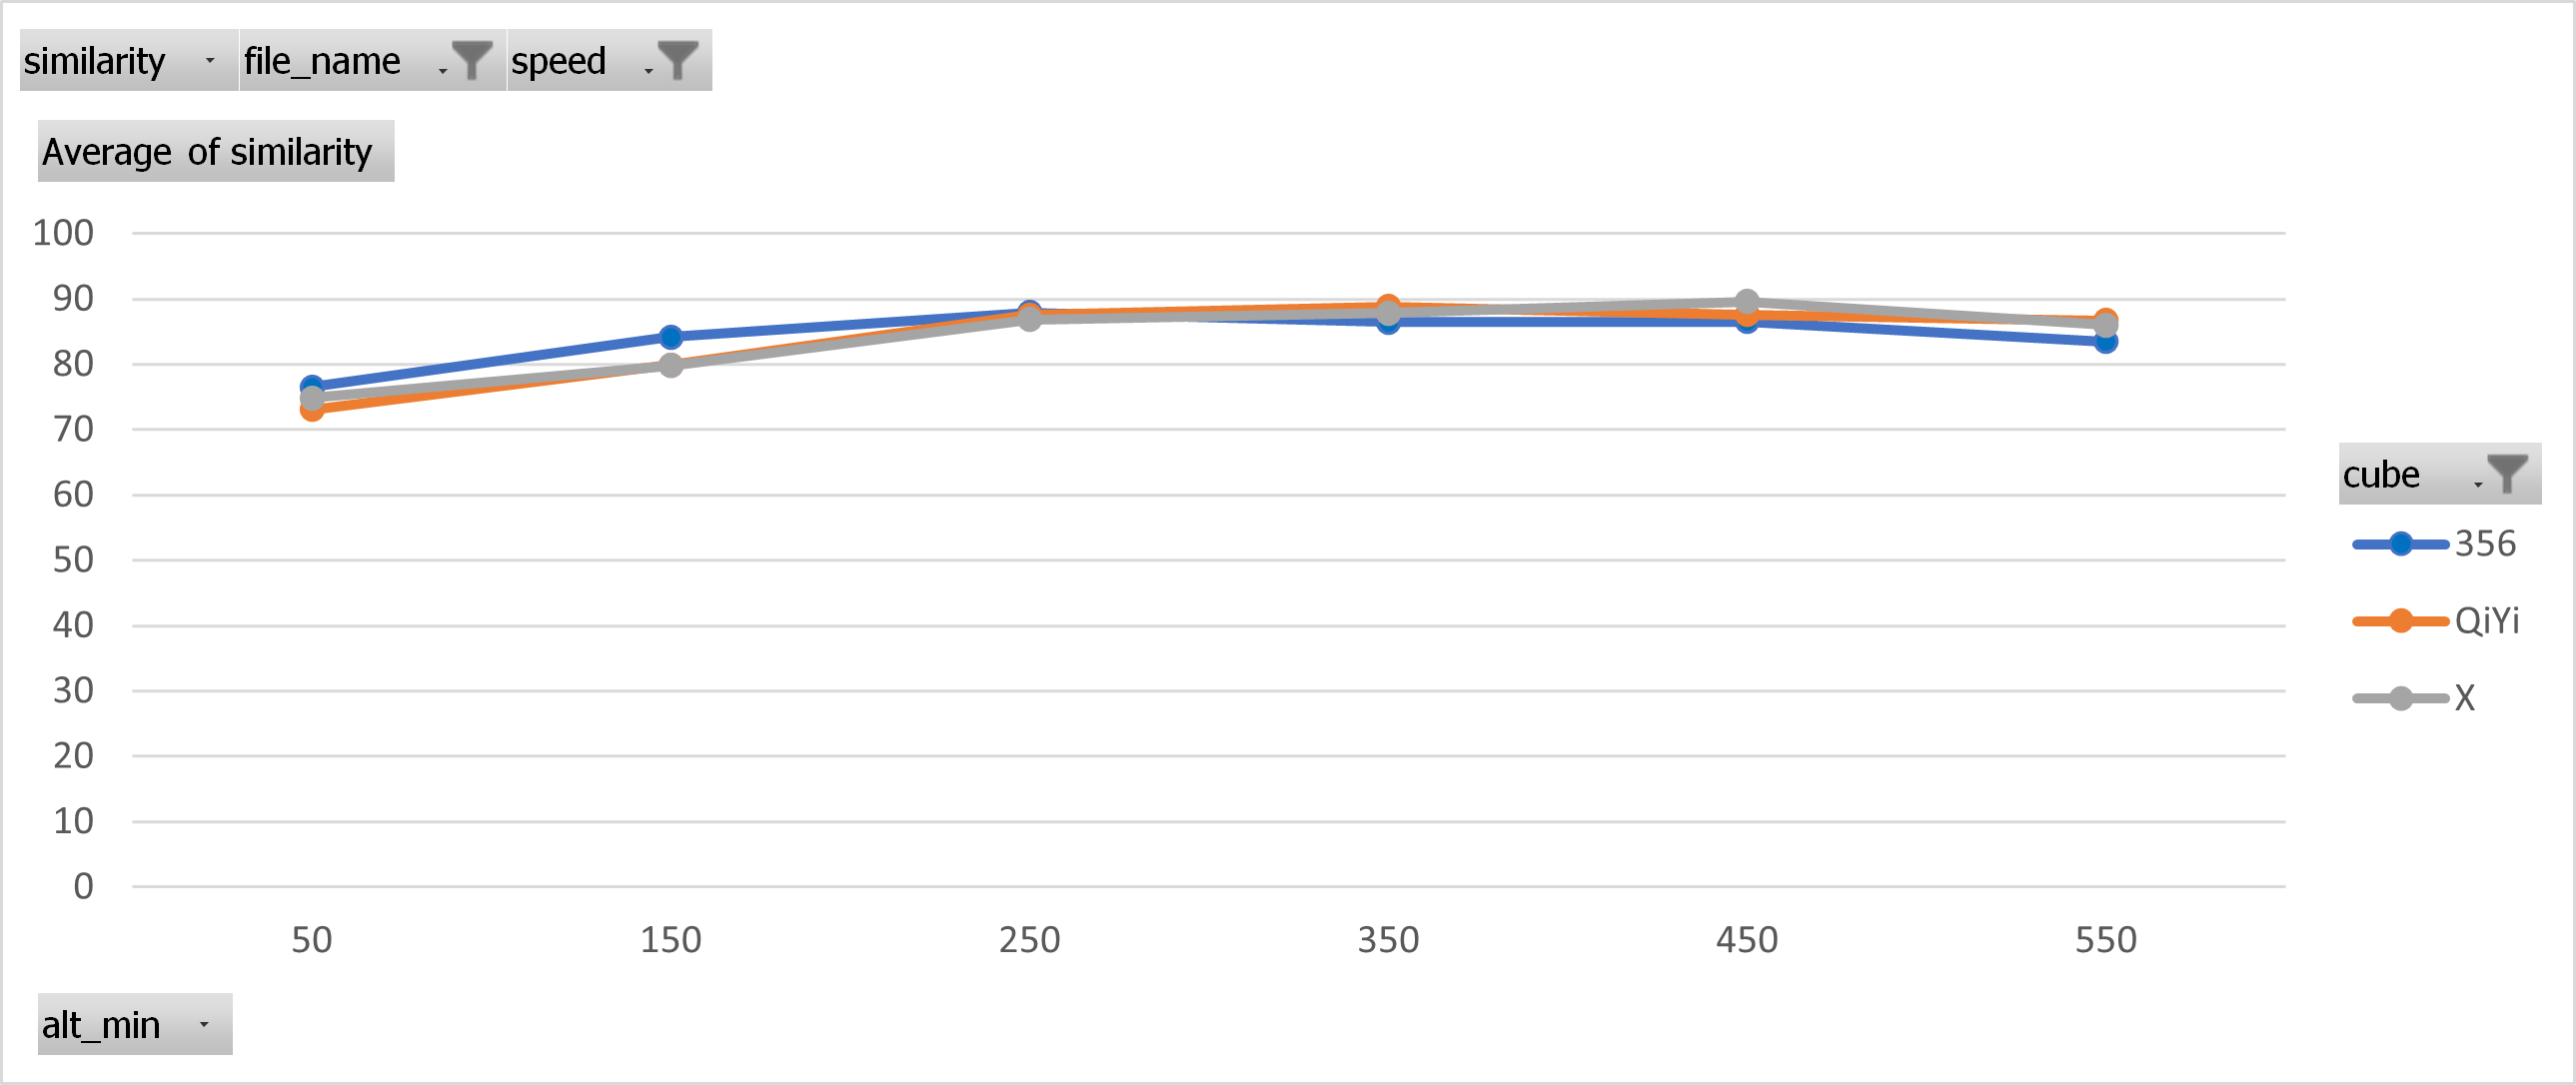
\includegraphics[width=\linewidth]{Figures/7 Evaluation/similarity_by_alt_min_5tps.png}
        \vspace*{.1mm}
    \end{subfigure}\\
\end{figure}


\subsection{Influence of Window Size}
\label{subsec:influence-window-size}

The final parameter tested in this experiment was the size of the
sliding window used to ensure that detected face turns had stabilized
before accepting them as real face turns. Since erroneous detections
rarely last for more than a few time steps, a higher window size was
expected to correspond to a higher detection accuracy.

Figure \ref{fig:influence-window-size} clearly shows that a window size
of five to ten time steps was consistently correlated with a higher
accuracy of detection. In fact, at 2 TPS, a window size of five to ten
corresponded to a nearly perfect \emph{average} detection for all
cubes, across the wide variation in the threshold parameters.

Furthermore, Figure \ref{fig:influence-window-size-average-5tps} shows
that a window size between five and eight time steps corresponded to
>90\% detection accuracy across all variations in the threshold
parameters, three to ten percentage points higher than the best
averages achieved by either threshold parameter.

\begin{figure}
    \caption{Perfect Detections by Window Size}
    \label{fig:influence-window-size}
    \begin{subfigure}{\textwidth}
        \centering
        \caption{Total number of perfect detections}
        \label{fig:perfect-detections-by-window-size-total}
        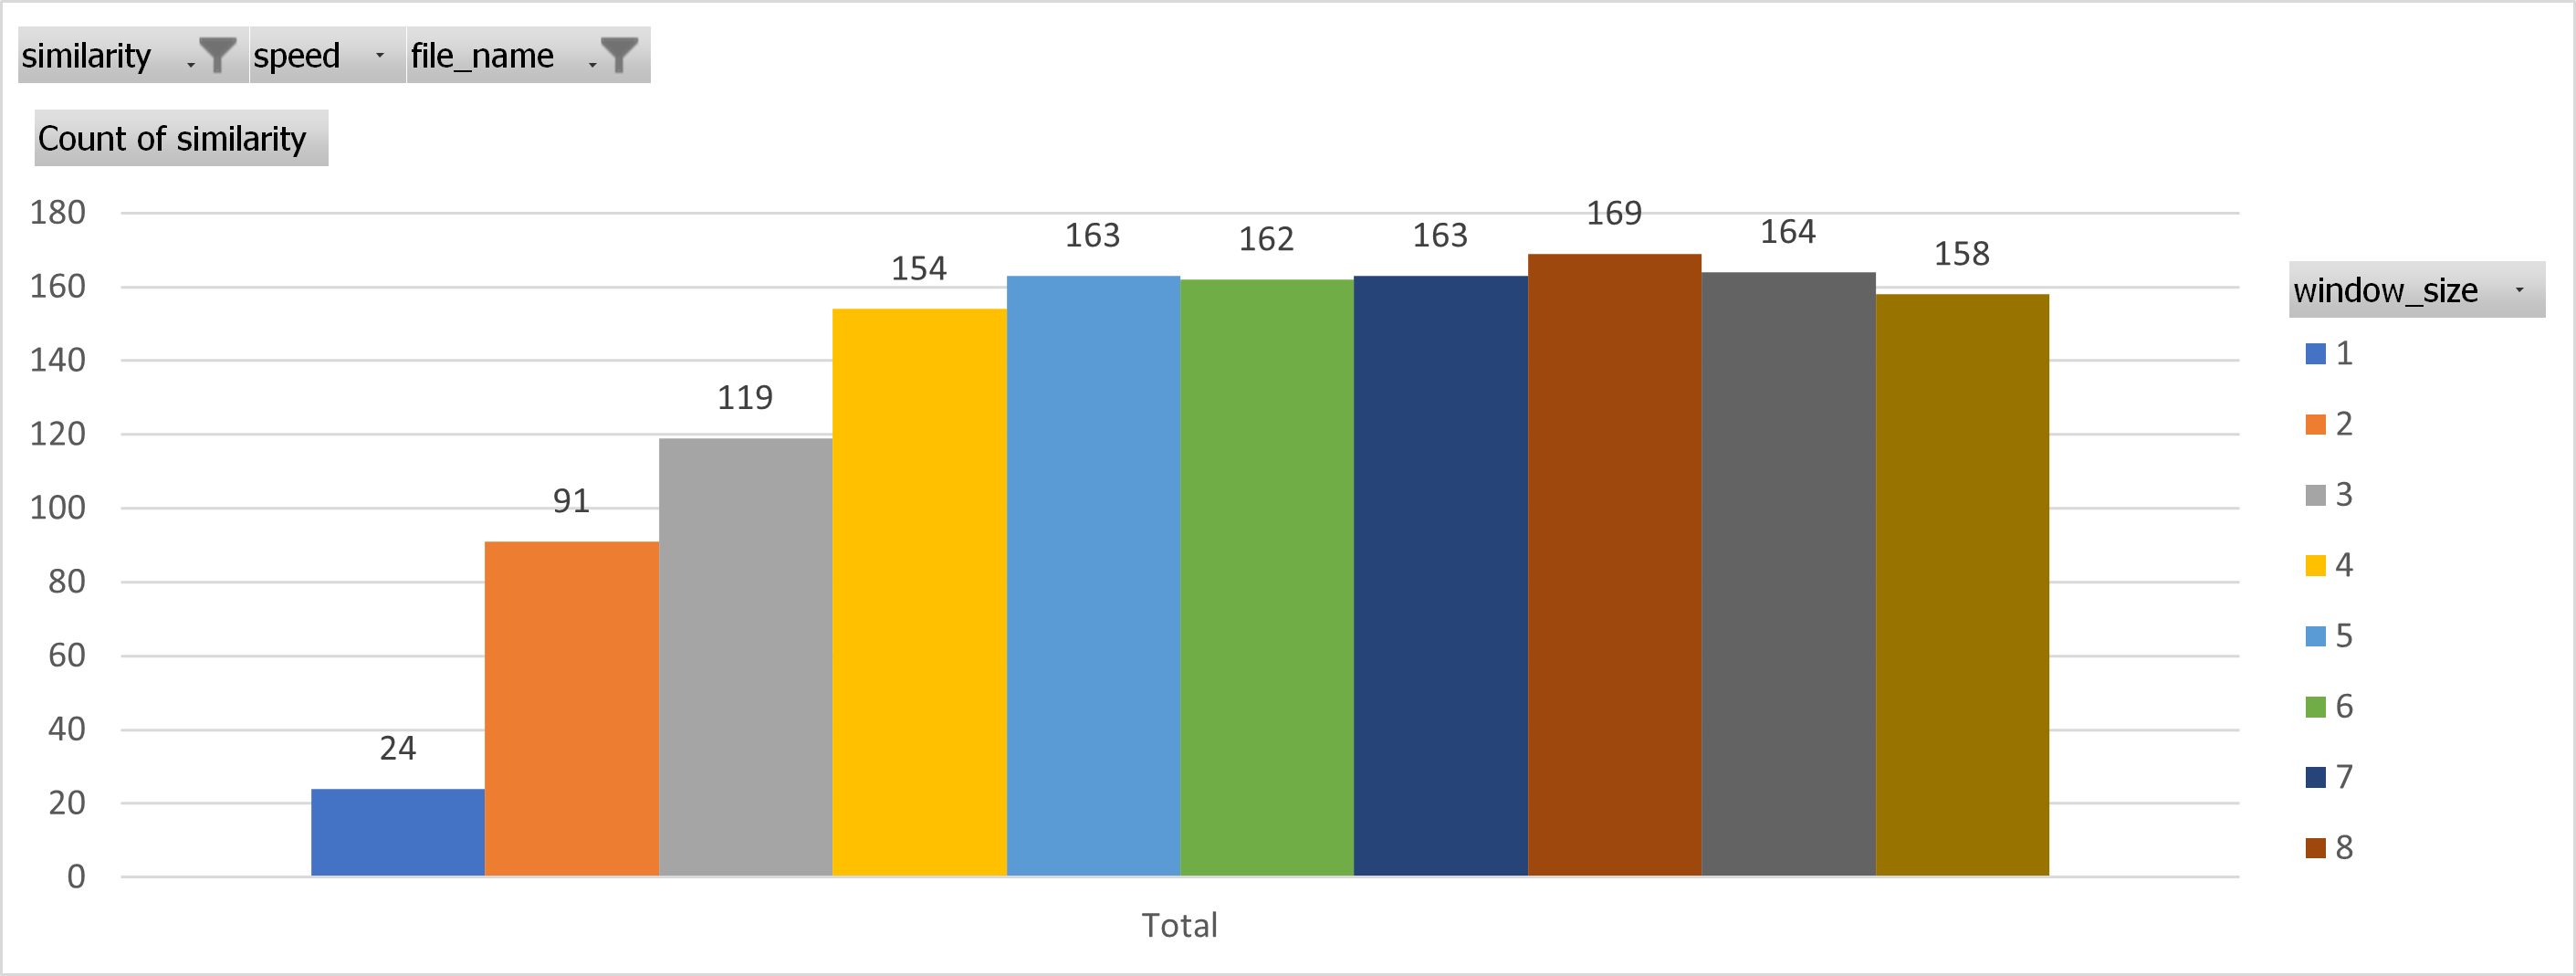
\includegraphics[width=\linewidth]{Figures/7 Evaluation/perfect_detections_by_window_size.png}
        \vspace*{.1mm}
    \end{subfigure}\\
    \begin{subfigure}{\textwidth}
        \centering
        \caption{Average Accuracy by Window Size at 2 TPS}
        \label{fig:influence-window-size-average-2tps}
        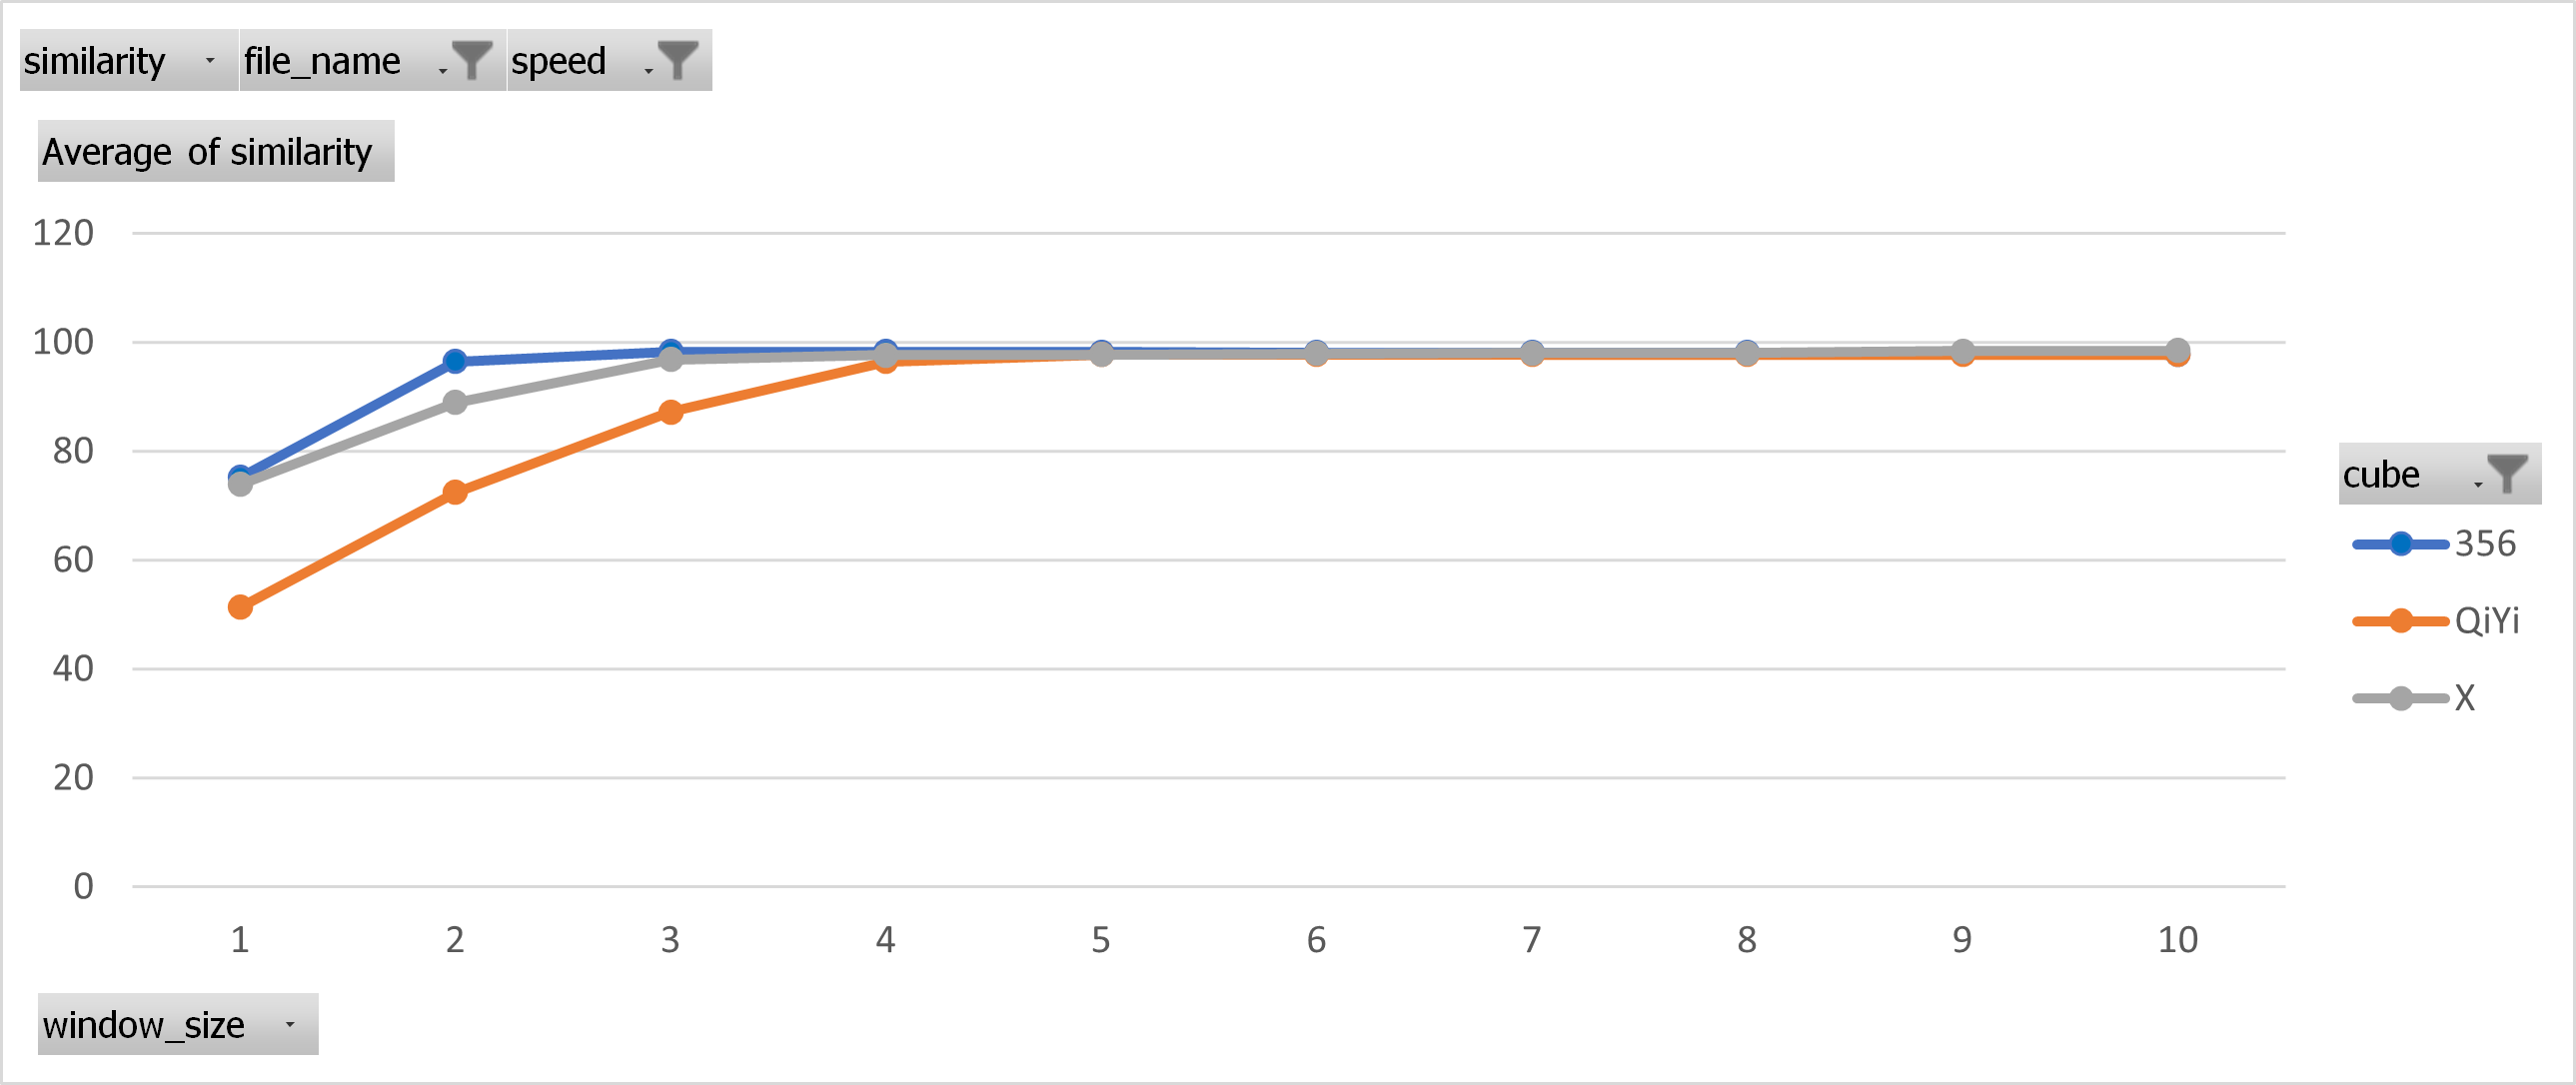
\includegraphics[width=\linewidth]{Figures/7 Evaluation/similarity_by_window_size_2tps.png}
        \vspace*{.1mm}
    \end{subfigure}\\
    \begin{subfigure}{\textwidth}
        \centering
        \caption{Average Accuracy by Window Size at 5 TPS}
        \label{fig:influence-window-size-average-5tps}
        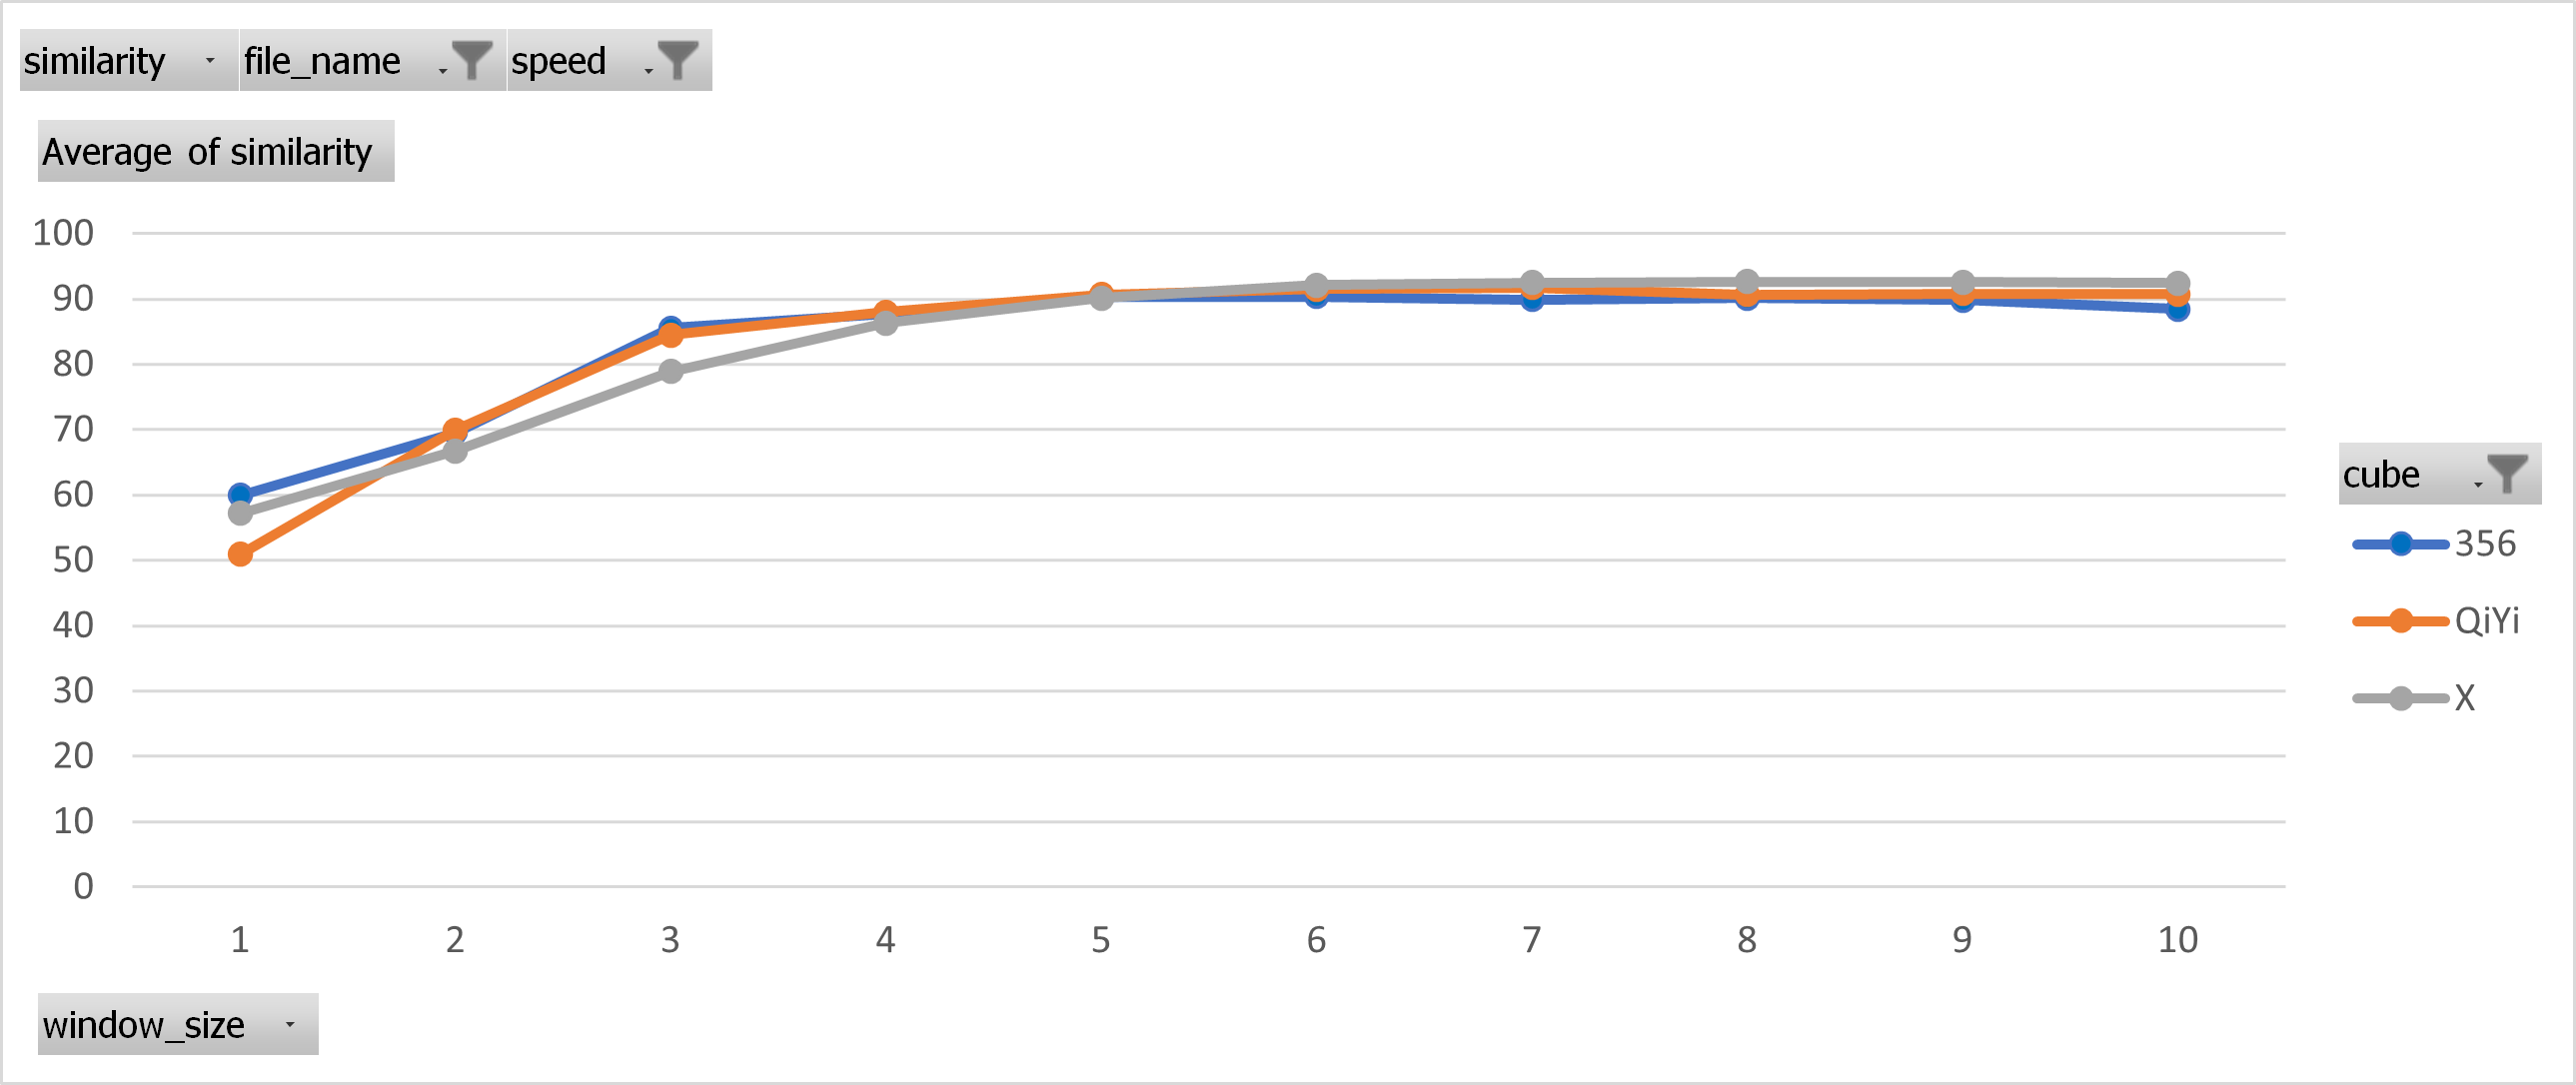
\includegraphics[width=\linewidth]{Figures/7 Evaluation/similarity_by_window_size_5tps.png}
        \vspace*{.1mm}
    \end{subfigure}\\
\end{figure}


\section{Compatibility with Standard Speedcubes}
\label{sec:compatibility-with-standard-speedcubes}

Since a major goal of this research project is to allow speedcubers to
practice with the same cube they compete with, it is imperative that
the proposed design function without requiring permanent modifications
to the original speedcube. For the same reason, the design must also
retain the original performance of the speedcube as much as possible.

As shown in Figure \ref{fig:core-placement}, the proposed PCB
transmitter can be deployed in a Gans 356 speedcube by simply changing
out the original centercap for a custom-built one containing the
transmitter. The modifications to the cube are purely temporary since
the original cube can be perfectly restored by simply replacing the
original centercaps.

The performance impact of the custom centercaps with the transmitters
is also small since the little weight they add to the cube is placed
close to the axes of rotation. On the Gans 356, a stock centercap has a
mass of 0.6719 grams, while the custom centercap shown in Figure
\ref{sec:miniaturization} has a mass of 1.6905 grams. Multiplying the
approximately 1.2 gram difference per centercap by the six centercaps
on the cube results in a 7.2 gram increase in mass for the entire
speedcube for a total mass of 91.3104 grams. Since the stock Gans 356
has a mass of 84.1204 grams, this is only an 8.6\% increase in mass,
which is within the range of variation between different
speedcubes.\footnote{For example, the acclaimed MoYu WeiLong GTS3 M has
a mass of 92g \cite{moyu-thecubicle}. More information about the
variation in masses of different speedcubes can be found at
\href{https://www.thecubicle.com/collections/3x3-speed-cubes}{TheCubicle.com}.}
This additional weight does increase the moment of interia of each
face; however, this increase is small because the added weight placed
close to the axes of rotation. As such, the corresponding performance
penalty of the extra weight would be small.


\section{Move Tracking Granularity}
\label{sec:move-tracking-granularity}

While tracking the moves performed on the speedcube constitutes the
minimum viable functionality for a design, additional features make a
design a more useful solution to the speedcubing community. Of most
value is the ability to track the amount of time spent performing each
face turn; from that single metric many other highly valuable metrics
can be derived like TPS over time, and time spent completing each stage
of the solution.

Though not shown in the pretty printed algorithm from Section
\ref{subsec:ignoring-noise-when-extracting-move-sequences}, the
proposed software receiver also records the time stamp at which it
detected each face turn. By computing the difference between time
stamps, one can calculate the amount of time spent performing each
individual face turn. While not implemented in this design, a more
sophisticated software receiver could provide even more precise
measurements from the same source data by measuring the amount of time
between stable signals for each centerpiece state.

However, since this design does not include a gyroscope, it cannot
provide metrics about cube orientation over time like the highest-end
commercial smartcubes. As such, this design cannot be used to directly
report x, y, and z cube rotations, though sophisticated post-processing
heuristics could predict the location of such rotations with decent
accuracy.


\section{Competition Legality}
\label{sec:competition-legality}

As discussed in Section \ref{subsec:the-rise-of-smart-cubes},
speedsolving competitors cannot use any electronics or audio equipment
while solving the cube in competition. Since a major goal of this
research project is to allow speedcubers to practice with the same cube
they compete with, a design must either inherently comply with existing
competition rules against the use of electronics or must result in a
cube that can be easily modified to regain compliance.

While the design proposed in this thesis, certainly does not inherently
comply with the existing competition regulations since it requires
embedding electronics into the cube, it does result in a cube that can
be easily modified to regain compliance. As mentioned in Section
\ref{sec:compatibility-with-standard-speedcubes}, the only modification
to the cube is an interchangeable centercap that can be easily removed
and replaced with the original centercap to produce a perfectly
competition-legal cube.

Interestingly, the sound-based nature of this design provides a
potential compromise on the use of smartcubes in competition. As
mentioned at the end of Section \ref{sec:minimizing-sound-obstruction},
a sound-based transmitter only works at a short range and can easily be
rendered inaccessible to a competitor by scrambling cubes several
meters away from the competitors (especially in a different room), or
playing audio at the same frequencies as the transmitter. As such,
these properties of sound-based turn tracking could provide an avenue
in which smartcubes could be safely allowed in competitions to aid in
solve reconstructions without enabling competitors to spy on scrambles.

\section{Summary}

In summary, this chapter explored the effectiveness of the design
proposed in Chapters \ref{Chapter4}, \ref{Chapter5}, and \ref{Chapter6}
against four benchmarks derived from the research questions outlined in
Section \ref{sec:research-questions}.

The analysis of the receiver algorithm revealed many configurations
that enabled it to achieve a perfect detection accuracy on the test
samples. Most impactful in that detection was the usage of a high
\code{window\_size} which achieved accuracies of over 90\% across all
variations in the other parameters. Additionally beneficial is the
receiver's ability to detect the time between face turns which opens
the door to calculating useful metrics like TPS over time.

The analysis of the transmitter also found promising results. A rough
prototype of the PCB was small enough to fit into a single centercap
without requiring any permanent modifications to the cube. Furthermore,
since the centercap was interchangeable, the electronic components
impermissible in competition could easily be removed to return the cube
to a competition-legal state. In addition, the added mass of the
electrical components did not significantly increase the weight of the
puzzle, nearly retaining its original performance.
